% =============================================================
% DRAFT PAPER -- merged from the five standalone excerpts in this
% directory (methodology.tex, model_necessity_study.tex,
% prediction_horizon_study.tex, hardware_validation_section5.tex,
% shape_tracking_results.tex), assembled 2026-10-24.
%
% THIS IS A DRAFT, NOT A SUBMISSION-READY MANUSCRIPT. Scaffolding
% still in it, marked with "% TODO" throughout:
%   - Title, author list, affiliations: placeholders.
%   - Abstract and Introduction: stub prose, not yet written for
%     real -- they summarize what is below, they do not motivate
%     or position it against prior work.
%   - Discussion and Conclusion: stub prose, same caveat.
%   - Bibliography: 14 entries still carry "% VERIFY" notes for
%     volume/issue/page/DOI (unchanged from methodology.tex).
%   - 22 "% VERIFY" items remain inline from methodology.tex's own
%     passes (core-wire modulus, dipole moment, FD step size, J_p(z)
%     condition-number range, command-stream rate, triangle/U-shape
%     sub-dimensions, run-ordering generalization, R_P/t_P
%     calibration accuracy). None were resolved in this merge.
%   - The three tables carried over from prediction_horizon_study.tex
%     (originally written in a single-column `article` class because
%     they did not fit IEEEtran's narrow column) are converted here
%     to `table*` (double-column-spanning floats) as a draft
%     expedient. This has not been compiled -- no LaTeX toolchain is
%     available in this environment -- so verify layout before
%     submission; the original file's own comment recommended
%     prose-only merging instead of fighting column width, which was
%     not followed here in favor of keeping the quantitative tables.
%   - No vision-accuracy figure exists anywhere in the repo (noted
%     as a gap in every prior pass); still missing here.
%   - U-shape path: carries only its earlier n=5 campaign throughout
%     this draft. It was NOT part of the n=10 hardware extension
%     described in \S\ref{sec:shape-results}, and no new U-shape data
%     was collected when that section was written.
% =============================================================
\documentclass[journal]{IEEEtran}

\usepackage{amsmath}
\usepackage{amssymb}
\usepackage{amsfonts}
\usepackage{graphicx}
\usepackage{booktabs}
\usepackage{array}
\usepackage{tikz}
\usetikzlibrary{arrows.meta,positioning}

\begin{document}

% TODO: real title.
\title{Model Fidelity, Prediction Horizon, and Controller Choice in
Magnetically Actuated Continuum Beam Steering: A Hardware Study}

% TODO: real author list / affiliations / funding.
% TODO: affiliation, funding, and corresponding-author contact go in the \thanks block below.
\author{Author~Name\thanks{Placeholder affiliation/funding text.}}

\maketitle

% TODO: this abstract is a stub summarizing section content, not a
% written abstract. Rewrite with real motivation/contribution framing
% before any submission.
\begin{abstract}
We report a hardware study of closed-loop control for a magnetically
actuated, permanently magnetized continuum beam steered by a
manipulator-mounted permanent magnet. Two controllers --- a
matched-authority seven-coordinate inverse-Jacobian controller (INV-7)
and a delay-aware receding-horizon MPC with an exact nullspace
regularizer --- are compared across free-space shape-tracking paths
(rectangle, triangle, U-shape) and a vessel-navigation task, under
scheduled- and frozen-Jacobian conditions and, for MPC, two prediction
horizons ($N{=}15$, $N{=}1$). On the vessel task, contact-aware,
time-varying Jacobian modeling and longer prediction horizons are each
shown, by independent live-hardware and offline-mechanistic evidence, to
improve tracking through identifiable mechanisms rather than by
correlation alone. On the free-space shape-tracking task
($n{=}10$ runs/condition, 140 live runs), the horizon result generalizes
without qualification, while the controller-architecture and
Jacobian-scheduling results do not: each reverses sign between the
rectangle and triangle geometries, indicating that at least two of this
system's central design choices are geometry-dependent rather than
universal.
\end{abstract}

% TODO: real introduction -- motivation, prior work, contribution list.
% This paragraph only orients the reader to what follows; it does not
% yet argue why any of it matters or how it differs from prior
% magnetically steered continuum-robot work.
\section{Introduction}
\label{sec:intro}
This paper reports two linked experimental programs on the same
magnetically actuated continuum-beam platform (\S\ref{sec:system}):
a shape-tracking campaign on free-space paths (\S\ref{sec:shape-results})
and a vessel-navigation campaign (\S\ref{sec:model-necessity}--\S\ref{sec:hw-validation})
investigating whether contact-aware beam modeling and MPC's receding
horizon are mechanistically necessary or merely correlated with better
tracking. \S\ref{sec:system}--\S\ref{sec:experiments} define the shared
system model, controllers, and experimental protocol used by every
result that follows.

% =============================================================
% methodology.tex body (Sec. I-III), preamble/bibliography stripped.
% =============================================================

\section{System Modeling and Reference Generation}
\label{sec:system}

\subsection{System and Task Definition}
\label{sec:problem}

A flexible, permanently magnetized beam is advanced through a fixed
insertion point while a permanent magnet, carried by the end-effector of a
six-axis manipulator, shapes it through magnetic interaction. Given a
desired tip trajectory $p^\star(t)$, the control problem is to select
manipulator joint velocities and an insertion rate that drive the beam tip
along $p^\star(t)$, subject to the manipulator's velocity, acceleration
and joint-range limits, using only the beam shape observed by an external
camera.

The physical input to the beam is the actuating magnet's pose together
with the insertion length,
\begin{equation}
\theta = \big[\,p_a;\ \phi_a;\ \ell\,\big]\in\mathbb{R}^{7},
\label{eq:theta}
\end{equation}
$p_a\in\mathbb{R}^3$ the magnet position and $\phi_a\in\mathbb{R}^3$ a
minimal (axis--angle) parameterization of its orientation. Since the
magnet is rigidly mounted on the end-effector, $\theta$ is determined by
the six joint angles $q\in\mathbb{R}^6$ through the manipulator's forward
kinematics, so the quantity commanded and tracked at each control step is
the configuration
\begin{equation}
z = \big[\,q;\ L\,\big]\in\mathbb{R}^{7}, \qquad u=\dot z,
\label{eq:config}
\end{equation}
where $q$ is measured from the manipulator and $L$ is command-integrated
from the applied insertion rate (Sec.~\ref{sec:online}), not
independently sensed: the advancer is assumed to realize its commanded
length without slip or buckling, an assumption revisited in Limitations.
$u=\dot z$ (six joint velocities and one insertion rate) is the control
signal produced by both controllers of Sec.~\ref{sec:control}.

The beam is assumed to deform within a single, calibrated plane, an
assumption shared by the vision reconstruction of Sec.~\ref{sec:online}
and by the two-dimensional task projection introduced with the shared
control model in Sec.~\ref{sec:common}. The offline reference path
(Sec.~\ref{sec:planner}) is defined in a planner frame $\mathcal F_P$;
sensing, manipulator kinematics, and feedback control are all expressed
in the robot-base frame $\mathcal F_R$. A calibrated rigid transform maps
reference tip positions between them,
\begin{equation}
{}^{R}p_{\mathrm{des}} = {}^{R}R_P\,{}^{P}p_{\mathrm{des}} + {}^{R}t_P,
\label{eq:frame-fit}
\end{equation}
applied once, at startup, to every planner-frame target consumed
downstream. The measured tip position, the control Jacobian, and the task
projection are already expressed in $\mathcal F_R$ and are not further
transformed. All task-space quantities from Sec.~\ref{sec:common} onward
are expressed in $\mathcal F_R$ and the frame superscript is omitted.
% VERIFY: report the physical calibration accuracy of R_P/t_P (e.g.
% residual at held-out calibration points).

\subsection{Quasi-Static Magnetic Beam Model}
\label{sec:beam-model}

The beam is modeled as a Cosserat rod of inserted length $\ell$ and
circular cross section under a piecewise-constant-strain (PCS)
discretization~\cite{rucker2010geometrically,renda2018discrete}: the
centerline is divided into $n_s$ nodes, and the local strain $u(s)$ (one
torsion, two bending curvatures, body frame) is constant on each segment,
with linear-elastic cross-sectional stiffness
$K=\operatorname{diag}(GI_p,EI,EI)$, $G=E/(2(1+\nu))$. The beam is assumed
to reach mechanical equilibrium quickly relative to the control period, so
its shape at each instant is the static energy minimizer for the
instantaneous magnet pose --- the standard modeling choice at the
actuation bandwidths considered
here~\cite{kratchman2017guiding,wu2025closedloop}.

The beam carries a fixed (hard-magnetized) moment density $m(s)$, and the
actuating magnet is modeled as an ideal point-dipole source, valid at the
beam--magnet separations realized during path
following~\cite{fu2023magnetic,kratchman2017guiding}.
% VERIFY: report the min/max magnet-to-beam separation actually spanned
% by the reference paths.
Writing $\Delta=x-p_a$, $r=\lVert\Delta\rVert$, and
$\hat\Delta=\Delta/r$, the dipole field is
\begin{equation}
B(x;\theta) = \frac{\mu_0}{4\pi r^{3}}
\Big[3(\hat\Delta^{\top}m_a)\hat\Delta - m_a\Big],
\label{eq:dipole-field}
\end{equation}
and the magnetic potential energy, with the beam's world-frame moment at
arclength $s$ given by $R(s)m(s)$, is
\begin{equation}
W_m[u;\theta] = -\int_0^{\ell} \big(R(s)m(s)\big)\cdot
B\big(p(s);\theta\big)\,ds,
\label{eq:magnetic-energy}
\end{equation}
with $(p(s),R(s))$ the centerline pose from the rod reconstruction
equations $p'=Re_3$, $R'=R\hat u$, integrated from the insertion point.
The total potential energy is $\Pi=W_{el}+W_m$, where
$W_{el}=\tfrac12\int_0^\ell(u-u^\circ)^\top K(u-u^\circ)\,ds$ is the
elastic energy about rest strain $u^\circ$; the implemented model also
supports gravitational and lumen-contact energy terms, identically zero
for the free-space, horizontally supported configuration evaluated here
and given in full in the supplementary material. By the quasi-static
assumption, the beam shape at a given input is
\begin{equation}
u^{*}(\theta) = \operatorname*{arg\,min}_{u}\ \Pi(u;\theta),
\label{eq:equilibrium}
\end{equation}
solved by bound-constrained quasi-Newton minimization
(L-BFGS-B~\cite{byrd1995lbfgsb}) on analytic energy gradients, with
quasi-static continuation in $\ell$ (each insertion length warm-started
from the previous) to track the equilibrium branch physically reached by
incremental insertion. The regulated output used by the offline planner
is the tip pose $y(\theta)=[p(\ell);R(\ell)e_3]\in\mathbb{R}^6$; the
online controllers (Sec.~\ref{sec:control}) regulate only its position
component, projected into the task plane of Sec.~\ref{sec:common}.

\emph{Calibration.} The beam is a bimaterial composite (a stiffer core
wire, softer magnetized outer matrix); $E$ denotes the effective
(matrix-dominated) bending modulus, fit to $\approx2.5$\,MPa against
measured static deflection under a known magnet pose, with $\nu=0.49$ for
the matrix. Beam diameter, node count $n_s$, and the magnet's grade and
dimensions are manufacturer/geometric values (Table~\ref{tab:params}).
% VERIFY: core-wire modulus/Poisson ratio and weighting in the effective
% composite K; magnet dipole moment and beam magnetic moment density (or
% the calibration fit that produced them).

\subsection{Control Jacobian}
\label{sec:jacobian}

The planner (Sec.~\ref{sec:planner}) and controllers
(Sec.~\ref{sec:control}) require $J_b(\theta)=\partial y/\partial\theta$.
Rather than re-solving \eqref{eq:equilibrium} under finite perturbations,
$J_b$ is obtained by implicit differentiation of the equilibrium
condition: differentiating $\nabla_u\Pi(u^*;\theta)=0$ gives
\begin{equation}
\frac{\partial u^{*}}{\partial\theta} = -\,\Pi_{uu}^{-1}\,\Pi_{u\theta},
\label{eq:ift}
\end{equation}
with $\Pi_{uu},\Pi_{u\theta}$ the second derivatives of the total energy
at equilibrium (finite-differenced from the analytic gradient;
% VERIFY: FD step size),
and the beam Jacobian follows by the chain rule,
\begin{equation}
J_b(\theta) = \frac{\partial y}{\partial u}
\frac{\partial u^{*}}{\partial\theta}
+ \left.\frac{\partial y}{\partial\theta}\right\rvert_{u=u^{*}}
\in\mathbb{R}^{6\times7}.
\label{eq:jacobian-chain}
\end{equation}
This implicit route contrasts with the finite-difference Jacobian
in~\cite{kratchman2017guiding} and the shooting-based sensitivity
of~\cite{wu2025closedloop}. Composing with the manipulator's geometric
Jacobian $J_r(q)\in\mathbb{R}^{6\times6}$ (standard closed-form revolute
expressions~\cite{lynchpark2017modern} from the same calibrated
Denavit--Hartenberg parameters used for forward kinematics) gives the full
configuration-space Jacobian
$J(z)=J_b(\theta(z))\operatorname{blkdiag}(J_r(q),1)\in\mathbb{R}^{6\times7}$.
Both online controllers regulate tip position only, so they use its
position-only sub-block: with $E_p=[\,I_3\ \ 0_{3\times3}\,]$,
\begin{equation}
J_p(z) = E_p\,J(z)\in\mathbb{R}^{3\times7},
\label{eq:jp}
\end{equation}
precomputed once per reference sample (Sec.~\ref{sec:planner}) and reused
online, never re-differentiated live. A single external magnet provides
few independent steering directions, so $J_p(z)$ is rank-deficient over
much of the workspace --- comparable rank deficiency is reported for
related single-magnet systems~\cite{kratchman2017guiding}; quantitative
conditioning data along the evaluated paths are reported in the
supplementary material. % VERIFY: representative singular-value ratios /
% condition-number range of J_p(z) along the evaluated reference paths.
This motivates the explicit treatment of near-null directions in the
predictive controller (Sec.~\ref{sec:mpc}).

\subsection{Offline Reference Trajectory Generation}
\label{sec:planner}

A reference trajectory is generated offline in two stages and supplied to
both controllers as a feedforward term. Waypoint configurations
$\chi_j=[q;\ell]_j$ are obtained sequentially by nonlinear least squares
on
\begin{equation}
r(\chi_j) =
\begin{bmatrix}
\big(p_{\mathrm{tip}}(\chi_j)-p_{\mathrm{des},j}\big)/\tau_p\\[2pt]
\big(t_{\mathrm{tip}}(\chi_j)-t_{\mathrm{des},j}\big)/\tau_t\\[2pt]
\sqrt{w_c}\,\big(\chi_j-\chi_{j-1}\big)/d_c\\[2pt]
\sqrt{w_0}\,\big(\chi_j-\chi_0\big)/d_0
\end{bmatrix},
\label{eq:planner-residual}
\end{equation}
whose blocks are the tip position/tangent errors (tolerances
$\tau_p,\tau_t$), a continuity term against the previous waypoint (weight
$w_c$, scale $d_c$), and a regularizer holding the redundant configuration
near a nominal posture $\chi_0$ (weight $w_0$, scale $d_0$); waypoints are
warm-started sequentially from the previous solution, with restarts as
needed given the non-convexity of \eqref{eq:planner-residual}, and each
accepted solution is validated against the full nonlinear forward model.
At convergence $p_{\mathrm{tip}}(\chi_j)\approx p_{\mathrm{des},j}$, so the
desired and model-consistent tip targets coincide along the accepted
path; Sec.~\ref{sec:common} therefore uses a single symbol,
$p_{\mathrm{des},k}$, for this reference tip target.

The geometric path is then time-parameterized by reachability-based
time-optimal path
parameterization~\cite{bobrow1985timeoptimal,shinmckay1985minimumtime,phampham2018reachability}:
a backward pass computes the controllable set and a forward pass the
maximum feasible speed profile subject to per-joint and insertion
velocity/acceleration bounds, the resulting timing law smoothed by a
$C^2$ spline and its duration dilated to an exact multiple of the control
period $\Delta t$ so reference samples align with control ticks. The
stage yields, for each reference sample $k$, a reference configuration
$z_{\mathrm{ref},k}$ and reference rate $u_{\mathrm{ref},k}$.

\section{Feedback Control}
\label{sec:control}

Both controllers track the same offline reference
$\{z_{\mathrm{ref},k},u_{\mathrm{ref},k},p_{\mathrm{des},k}\}$
(Sec.~\ref{sec:planner}) and reuse $u_{\mathrm{ref},k}$ as feedforward,
correcting only the residual rather than re-deriving the trajectory
online.

\subsection{Common Delay-Aware Prediction Model}
\label{sec:common}

Tip position is regulated through a task-plane projector
$C\in\mathbb{R}^{2\times3}$ (the beam's axial and lateral in-plane
directions), giving the task Jacobian
$J_{\mathrm{task},k}=CJ_{p,k}\in\mathbb{R}^{2\times7}$ from the Jacobian
source $J_{p,k}$ defined below. Both controllers have real feedback
authority over all seven actuated coordinates --- six joints and
insertion --- under the same physical velocity/acceleration limits
(Table~\ref{tab:params}); this, not any particular normalization, is what
\emph{matched authority} refers to throughout this paper. On top of that
shared physical authority, both controllers are compared under the same
actuator normalization,
\begin{equation}
S_u = \operatorname{diag}\big(0.05,\dots,0.05,\,5\times10^{-3}\big)
\in\mathbb{R}^{7\times7}
\label{eq:su}
\end{equation}
(joints in rad/s, insertion in m/s), and
$S_z=\operatorname{diag}(0.5^{\circ},\dots,0.5^{\circ},\,0.25\text{mm})$
for configuration-space quantities; $S_u$ makes INV-7's seven-channel
allocation (Sec.~\ref{sec:inv7}) unit-consistent and gives the normalized
feedback-effort metric (Sec.~\ref{sec:metrics}) an identical,
controller-agnostic scale for both controllers.

\emph{Jacobian source.} Two conditions are compared as a robustness
stress test (Sec.~\ref{sec:protocol}):
\begin{align}
\text{Scheduled-}J\ \text{(SJ)}:&\quad J_{p,k} = J_{p,\mathrm{ref},k},
\label{eq:sj}\\
\text{Frozen-}J\ \text{(FJ)}:&\quad J_{p,k} = J_p(z_{\mathrm{ref},0})\ \forall k,
\label{eq:fj}
\end{align}
where $J_{p,\mathrm{ref},k}=J_p(z_{\mathrm{ref},k})$ is the schedule
\eqref{eq:jp} evaluated once, offline, at every reference sample. FJ holds
the initial reference Jacobian fixed for the entire run and is used as a
controlled model-staleness stress test; SJ is the intended operating
condition. Both controllers draw $J_{p,k}$ from the same source for a
given run, including the MPC's nullspace-projector construction
(Sec.~\ref{sec:mpc}): an FJ run freezes every quantity derived from $J_p$
together, not the prediction model alone.

\emph{Delay.} Both controllers account for a measured delay of $d=2$
control ticks between a newly issued joint-velocity command and its first
effect on the manipulator's commanded joint position (identified for the
six joints; the insertion advancer responds without this delay). Writing
$c_{k}$ for the joint-position command already committed at tick $k$ and
$u_{q,r|k}$ for the joint-rate command chosen for horizon stage $r$ at
tick $k$,
\begin{equation}
q^{\mathrm{phys}}_{j|k} =
\begin{cases}
c_{k-1}, & j=1,\\
c_{k}, & j=2,\\[2pt]
\displaystyle c_{k} + \Delta t\sum_{r=0}^{j-3}u_{q,r|k}, & j=3,\dots,N,
\end{cases}
\label{eq:delay-stages}
\end{equation}
so stage $j{=}3$ is the first predicted stage the newly optimized command
$u_{q,0|k}$ can affect, and every later stage accumulates all joint
commands decided so far in the horizon; stages $j{=}1,2$ are already
committed. Insertion integrates without this offset,
$L_{j|k}=L_k+\Delta t\sum_{r=0}^{j-1}u_{L,r|k}$. This is why the
mechanistic evaluation and horizon ablation (Sec.~\ref{sec:replay}) are
stated at the $+3$ stage, and why the minimum causally responsive horizon
is $N=3$.

\emph{Persistent output-disturbance prediction.} A per-tick
output-disturbance estimate,
\begin{equation}
d_k = C p_{\mathrm{meas},k} -
\Big[C p_{\mathrm{des},k} +
J_{\mathrm{task},k}\big(z_{\mathrm{meas},k}-z_{\mathrm{ref},k}\big)\Big]
\in\mathbb{R}^2,
\label{eq:residual}
\end{equation}
is formed for the MPC's horizon prediction and, at its own preview index,
by INV-7 (Sec.~\ref{sec:inv7}); the same residual is reused offline as a
common evaluator for both controllers' recorded runs
(Sec.~\ref{sec:replay}). Writing $\delta z_{j|k}=z^{\mathrm{phys}}_{j|k}-z_{\mathrm{ref},k+j}$,
the MPC prediction holds $d_k$ fixed across the horizon,
\begin{align}
\hat p_{j|k} &= C p_{\mathrm{des},k+j}
+ J_{\mathrm{task},k+j}\,\delta z_{j|k}
+ \beta_d\,d_k,
\label{eq:disturbance-prediction}\\
\beta_d &= 1,\notag
\end{align}
i.e.\ it assumes the observed model-mismatch persists rather than
decaying. We call this \emph{persistent output-disturbance prediction}
rather than ``offset-free'' tracking: \eqref{eq:residual} is a per-tick
estimate, not an integrated state, and carries no guarantee of zero
steady-state error for the nonlinear plant.

\subsection{Matched-Authority Inverse-Jacobian Controller (INV-7)}
\label{sec:inv7}
INV-7 (named for its seven actuated coordinates) is delay-aware through a
one-shot preview rather than the committed-command propagation
\eqref{eq:delay-stages} used by the receding-horizon MPC. Let $r_k$ be the
runtime-logged reference index at tick $k$ and define the realization
index
\begin{equation}
\kappa_k = r_k+1+d,
\label{eq:kappa}
\end{equation}
the same $+3$ causal offset as \eqref{eq:delay-stages}: the first
reference sample tick $k$'s decision can affect. The current-tick residual
\eqref{eq:residual} is formed at $r_k$. The preview joint configuration is
read directly from the reference trajectory at $\kappa_k$ (not propagated
from INV-7's own recent commands), concatenated with a feedforward-only
insertion preview $\ell_k$ ($\ell_{k+1}=\ell_k+\Delta t\,u_{L,\mathrm{ref},k}$,
undelayed):
\begin{equation}
\hat z_{\kappa_k|k} = \big[\,z_{\mathrm{ref},\kappa_k}[1{:}6];\ \ell_k\,\big].
\label{eq:inv7-preview-state}
\end{equation}
$\ell_k$ is only this preview \emph{base}; insertion still receives
feedback like the six joints, through the insertion component of the trim
$\delta z_k$ below, applied to $\hat z_{\kappa_k|k}$ before the command is
realized (Sec.~\ref{sec:online}). With the preview task Jacobian
$J_{\mathrm{task},\kappa_k}=CJ_{p,\kappa_k}$ (evaluated at $\kappa_k$, from
the SJ/FJ source of Sec.~\ref{sec:common}),
\begin{align}
\hat p_{\kappa_k|k} &= C p_{\mathrm{des},\kappa_k} +
J_{\mathrm{task},\kappa_k}\big(\hat z_{\kappa_k|k}-z_{\mathrm{ref},\kappa_k}\big)
+ d_k,
\label{eq:inv7-preview-error}\\
e_{\kappa_k|k} &= C p_{\mathrm{des},\kappa_k} - \hat p_{\kappa_k|k}.
\notag
\end{align}
With $J_{u,\kappa_k}=J_{\mathrm{task},\kappa_k}S_u$ the normalized preview
task Jacobian, the correction is a normalized damped-least-squares
step~\cite{nakamura1986inverse,wampler1986manipulator},
\begin{align}
J_{u,\kappa_k}^{+} &= J_{u,\kappa_k}^{\top}
\big(J_{u,\kappa_k}J_{u,\kappa_k}^{\top}+\lambda_u^2 I\big)^{-1},
\qquad \lambda_u = 2.5\times10^{-3},
\label{eq:inv7-pinv}\\
\delta z_k &= S_u\Big(J_{u,\kappa_k}^{+}\,k_p\,e_{\kappa_k|k}\Big),
\qquad k_p=1,
\notag
\end{align}
$\lambda_u$ trading tracking accuracy against command magnitude near
singularities~\cite{chiaverini1994review}; $\delta z_k$ is a physical-unit
configuration trim, not a rate. No redundancy/posture regularization is
applied ($k_n=0$): $u_{\mathrm{ref},k}$ carries the entire nominal
(including planned insertion) motion. The command is realized as an
absolute position trim, the same accumulator mechanism as MPC
(Sec.~\ref{sec:online}): the persistent commanded configuration $c_k$ is
advanced toward $\hat z_{\kappa_k|k}+\delta z_k$, clipped componentwise to
the physical rate/acceleration limits, and the clipped step divided by
$\Delta t$ is issued. INV-7 draws $J_{p,\kappa_k}$ from the SJ/FJ source
(never from $z_{\mathrm{meas},k}$ directly) and runs in-process, a single
closed-form solve per tick.

\subsection{Delay-Aware Output-Tracking MPC}
\label{sec:mpc}
The predictive controller optimizes a horizon of $N=15$ rate commands
$U=[u_{0|k};\dots;u_{N-1|k}]$ against \eqref{eq:delay-stages}--\eqref{eq:disturbance-prediction},
with $u_{-1|k}=u_{k-1}$ (the previously applied command) so the rate
constraint below is well-defined at $j=0$, and an \emph{exact}
nullspace-only configuration regularizer in place of a full-state weight.
At horizon stage $j$, let $J_{s,j|k}=J_{\mathrm{task},k+j}S_z$ and
\begin{equation}
J_{s,j|k}=U_{j|k}\Sigma_{j|k}\big[\,V_{r,j|k}\ \ V_{n,j|k}\,\big]^{\top},
\qquad P_{N,j|k}=V_{n,j|k}V_{n,j|k}^{\top},
\label{eq:pn}
\end{equation}
its full singular value decomposition, $V_{n,j|k}$ spanning the numerical
null space: a full, rank-revealing SVD is used so that $P_{N,j|k}$ is an
exact orthogonal null-space projector, constructed fresh at every stage.
Writing $\tilde z_{j|k}=S_z^{-1}\delta z_{j|k}$ and
$\Delta u_{j|k}=u_{j|k}-u_{j-1|k}$, the command is the solution of
\begin{subequations}
\label{eq:mpc}
\begin{align}
\min_{U}\quad &
\sum_{j=1}^{N}\big\lVert \hat p_{j|k}-Cp_{\mathrm{des},k+j}\big\rVert^2_{Q_p}
+ \sum_{j=0}^{N-1}\big\lVert u_{j|k}-u_{\mathrm{ref},k+j}\big\rVert^2_{R}
\notag\\
&\ + \sum_{j=0}^{N-1}\big\lVert \Delta u_{j|k}\big\rVert^2_{R_d}
+ \sum_{j=1}^{N}\big\lVert P_{N,j|k}\,\tilde z_{j|k}\big\rVert^2
\label{eq:mpc-objective}\\
\text{s.t.}\quad & u_{\min}\le u_{j|k}\le u_{\max},
\label{eq:mpc-input}\\
& \Delta u_{\min}\le \Delta u_{j|k}\le \Delta u_{\max},
\label{eq:mpc-rate}\\
& z_{\min}\le z^{\mathrm{phys}}_{j|k}\le z_{\max}.
\label{eq:mpc-state}
\end{align}
\end{subequations}
All inequalities are componentwise; \eqref{eq:mpc-input}--\eqref{eq:mpc-rate}
apply for $j=0,\dots,N-1$ and \eqref{eq:mpc-state} for $j=1,\dots,N$. The
program is solved by operator splitting~\cite{osqp2020}, of which only
$u_{0|k}$ is applied before the horizon recedes. $Q_p$ weights tip-output
tracking at a $0.5$\,mm error scale (weight $1.0$) and is the primary
objective. $R$ and $R_d$ use two separate normalization scales, $S_u$
\eqref{eq:su} and a distinct increment scale
$S_{\Delta u}=\operatorname{diag}(0.04,\dots,0.04,\,2\times10^{-3})$
rad/s ($\times6$), m/s, giving
\begin{equation}
R = 7.0\,S_u^{-\top}S_u^{-1}, \qquad
R_d = 1\times10^{-3}\,S_{\Delta u}^{-\top}S_{\Delta u}^{-1}.
\label{eq:r-rd}
\end{equation}
Only null-space configuration error is penalized: the configuration
regularizer contains no row-space component, while $R$ and $R_d$ remain
active in all directions, including row-space (task-relevant) motion. The
null-space term discourages drift, at each stage's own linearization, in
directions locally task-null to first order; it does not guarantee the
corresponding motion remains task-null over a finite step, a distinction
explored directly in a manipulability-objective investigation reported in
the supplementary material. There is no terminal cost, terminal set, or
directional damping term, and no nominal stability guarantee is claimed
for the nonlinear plant. INV-7 enforces the same bounds as a sequence of
post-hoc limits on an already-computed command; MPC enforces them as hard
constraints in \eqref{eq:mpc}.

\section{Experimental Methods}
\label{sec:experiments}

\subsection{Vision and Real-Time Control}
\label{sec:online}

An overhead camera tracks colored fiducials on the beam (base, one or
more intermediate points, and tip), segmented by HSV thresholding and
localized by centroid; three proximal markers define a local beam-plane
frame by principal component analysis, each marker is projected into it
and scaled to metric units by a fixed reference pair of known separation,
and a calibrated rigid transform maps the result into the robot frame.
Reconstruction runs on a dedicated thread, unfiltered, decoupled from the
control loop, which consumes the most recent estimate each tick.

Both controllers realize their commanded rate through a shared mechanism:
a persistent, controller-owned absolute command $c_k$, advanced each tick
as $c_{k+1}=c_k+\Delta t\,u_k$ and interpolated at the manipulator's
command-stream rate, rather than isolated per-tick velocity impulses. The
insertion component of this accumulator is clipped to a physically
realizable range at every update and is the sole source of the
controller's insertion state; it is never corrected from the
vision-derived beam length. INV-7's command is a single closed-form
solve per tick; the MPC solve was executed in a pre-warmed,
process-isolated worker with a 70\,ms per-tick deadline, holding the
previously committed position on a missed deadline rather than applying a
stale solve. Runs were automatically terminated on stale vision,
solver/worker failure, a manipulator protective stop, a non-finite
command, or violation of a predeclared Cartesian workspace bound on the
measured tool-center-point position --- bounds tight enough to
auto-terminate a divergent run (Sec.~\ref{sec:protocol}) without manual
intervention. Platform and timing parameters are in
Table~\ref{tab:hardware}, model/controller parameters in
Table~\ref{tab:params}.

\subsection{Experimental Protocol}
\label{sec:protocol}

The two controllers are compared on three path geometries (rectangle,
triangle, U-shape; nominal dimensions in Table~\ref{tab:params}), using
the beam and platform of Sec.~\ref{sec:beam-model}--\ref{sec:online}.
Controller parameters are fixed once and not retuned between geometries,
licensing the three geometries as a generalization check on a single
design rather than three separately tuned instances. The rectangle and
triangle paths carry the full campaign described below; the U-shape path
retains the smaller $n=5$ campaign of an earlier round and is reported
separately with its own sample size, not pooled with the rectangle/triangle
results.

The primary comparison is INV-7 vs.\ MPC under scheduled-$J$
(Sec.~\ref{sec:common}), 10 repeated live runs per controller and path on
the rectangle and triangle (5 on the U-shape; the run, not the tick, is
the experimental unit, Sec.~\ref{sec:metrics}). A second, factorial
comparison crosses controller with Jacobian condition (SJ, FJ) on the
rectangle and triangle paths, again 10 repeated runs per cell, as a
robustness stress test to model staleness. A third comparison, run only
on MPC, crosses Jacobian condition (SJ, FJ) with prediction horizon
$N\in\{15,1\}$ on the rectangle and triangle paths, 10 repeated runs per
cell, isolating the horizon's own contribution from the Jacobian-source
comparisons; this complements, and is reported alongside, the offline
decision-level horizon ablation of Sec.~\ref{sec:replay} with an
independent live-hardware result at the two horizon extremes actually
used elsewhere in this protocol. On the U-shape path, both attempted
MPC-FJ trials developed rapidly increasing tracking error in the same
path region and were safety-terminated (Sec.~\ref{sec:online}) before
completing the path; no complete-path metric is reported for that cell,
and it is reported as a genuine failure mode rather than omitted or
imputed.

Each run starts from the same calibrated home configuration, after the
frame transform \eqref{eq:frame-fit} and workspace bounds are
(re-)verified; the reference trajectory, actuator limits, and control
period are identical across controllers and conditions for a given path.
On the rectangle path, the two controllers' runs for a given Jacobian
condition were collected as separate blocks (all MPC-SJ, then all MPC-FJ;
all INV-7-SJ and INV-7-FJ runs interleaved with each other), all within a
single session, and no controller-order effect is assumed without
checking for one. % VERIFY: confirm and generalize this run-ordering
% description to the triangle and U-shape sessions, and state the
% inter-run reset procedure beyond returning to the home configuration.

\subsection{Evaluation Metrics and Statistical Analysis}
\label{sec:metrics}

Every per-tick error uses the runtime-logged reference index $r_k$
(Sec.~\ref{sec:inv7}), not an assumed tick-to-sample correspondence:
\begin{equation}
e_k = C\big(p_{\mathrm{meas},k}-p_{\mathrm{des},r_k}\big).
\label{eq:tick-error}
\end{equation}
Tracking accuracy is the run-level RMS of \eqref{eq:tick-error},
\begin{equation}
E_{\mathrm{RMS}} = \sqrt{\tfrac1T\textstyle\sum_{k=1}^{T}\lVert e_k\rVert^2},
\label{eq:e-rms}
\end{equation}
decomposed by axis as $E_{x,\mathrm{RMS}}$, $E_{y,\mathrm{RMS}}$.
Feedback effort is the run-level RMS of the $S_u$-normalized deviation
from feedforward,
\begin{equation}
E_u = \sqrt{\tfrac1T\textstyle\sum_{k=1}^{T}
\big\lVert S_u^{-1}\big(u_k-u_{\mathrm{ref},r_k}\big)\big\rVert^2},
\label{eq:e-u}
\end{equation}
dimensionless, on the same $S_u$ for both controllers. Two
constraint-activity fractions are reported, each the fraction of
evaluated ticks at which the corresponding bound of \eqref{eq:mpc} is
active to within a numerical tolerance of $10^{-6}$: \emph{insertion
velocity-limit activity} \eqref{eq:mpc-input}, and \emph{joint
command-increment (acceleration-limit) activity} \eqref{eq:mpc-rate} ---
the joint velocity bound itself is rarely approached.

The independent experimental unit is the \emph{run}: with
$T\!\approx\!250$--$290$ ticks per run and $n=10$ runs per condition on
the rectangle and triangle paths ($n=5$ on the U-shape, unchanged from
the earlier round), tables report run-level mean$\,\pm\,$95\% confidence
interval, $\bar x\pm t_{0.975,n-1}\,s/\sqrt n$ ($t_{0.975,9}\approx2.262$
at $n=10$, $t_{0.975,4}\approx2.776$ at $n=5$), computed from the
run-level values, not the $\approx\!2500$--$2900$ pooled
(non-independent) ticks at $n=10$. Group comparisons additionally use the
two-sided Mann-Whitney $U$ test on the $n$ run-level RMSE values, which
makes no normality assumption and is reported alongside the CI for every
primary comparison. Figures show individual run-level points together
with the run-level mean and this same confidence interval. Tick-resolved
traces are used only for time/path-resolved visualization and the
mechanistic analyses of Sec.~\ref{sec:replay}, not as additional
statistical samples. Cross-geometry claims are stated as heterogeneous in
effect size (large on the rectangle, smaller on the triangle, and not yet
re-established at $n=10$ on the U-shape) rather than as a uniform effect.

\subsection{Offline Mechanistic Replay and Ablations}
\label{sec:replay}

Two further analyses are computed offline against recorded runs, using
\eqref{eq:residual} applied identically regardless of which controller or
Jacobian source produced the recorded command --- a common evaluator. For
a recorded tick with logged command $u_{0|k}$ and feedforward
$u_{\mathrm{ref},k}$, the model predicts the causal $+3$ task-plane error
twice: with the logged command, $\hat e_{3|k}$, and with
$u_{\mathrm{ref},k}$ substituted (``no new correction''),
$\hat e_{3|k}^{\,\mathrm{base}}$, both through
\eqref{eq:disturbance-prediction} with the same logged $d_k$. A correction
is \emph{useful} when
$\lvert e_y\rvert^{\mathrm{base}}_{3|k}-\lvert e_y\rvert_{3|k}>0$; the
directional-reliability metrics are the fraction of ticks meeting this,
\begin{equation}
P(\text{useful}_y{>}0) =
\tfrac1K\textstyle\sum_k \mathbb{1}\big[\lvert e_y\rvert^{\mathrm{base}}_{3|k}
-\lvert e_y\rvert_{3|k}>0\big],
\label{eq:p-useful}
\end{equation}
and the signed aggregate net correction per unit normalized joint effort,
\begin{equation}
\eta_{y,\mathrm{net}} =
\frac{\sum_k\big(\lvert e_y\rvert^{\mathrm{base}}_{3|k}-\lvert e_y\rvert_{3|k}\big)}
{\sum_k\big\lVert S_{u,q}^{-1}(u_{q,0|k}-u_{q,\mathrm{ref},k})\big\rVert},
\label{eq:eta-y}
\end{equation}
where harmful corrections (negative numerator terms) are counted, not
discarded. The numerator is lateral ($y$) task correction while the
denominator is joint effort specifically: this metric isolates the
lateral magnetic-steering efficiency examined in the mechanism analysis,
and insertion's own contribution to lateral correction is small in the
actuator decomposition (supplementary).

The same recorded-tick replay is also used for two targeted ablations on
the rectangle path: (i) disabling persistent-disturbance prediction
($\beta_d=0$ vs.\ the validated $\beta_d=1$) and re-evaluating the $+3$
predicted error, paired per recorded trajectory; and (ii) sweeping the
prediction horizon $N\in\{3,5,10,15\}$ and comparing the resulting
$u_{q,0}$ by cosine similarity against its $N{=}15$ value. These replays
quantify short-horizon decision-level counterfactual effects from
recorded states; they are not alternative realized closed-loop hardware
trajectories, and are not treated as equivalent to an additional live-run
comparison.

\begin{figure}[t]
\centering
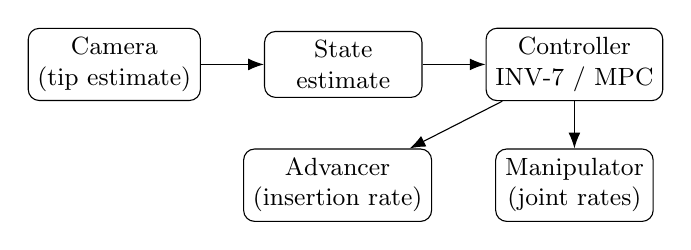
\begin{tikzpicture}[
  node distance=6mm and 8mm,
  box/.style={draw, rounded corners, align=center, minimum height=8mm, minimum width=20mm, font=\small},
  >={Latex[length=2mm]}
]
\node[box] (cam) {Camera\\(tip estimate)};
\node[box, right=of cam] (state) {State\\estimate};
\node[box, right=of state] (ctrl) {Controller\\INV-7 / MPC};
\node[box, below=of ctrl] (robot) {Manipulator\\(joint rates)};
\node[box, left=of robot] (adv) {Advancer\\(insertion rate)};
\draw[->] (cam) -- (state);
\draw[->] (state) -- (ctrl);
\draw[->] (ctrl) -- (robot);
\draw[->] (ctrl) -- (adv);
\end{tikzpicture}
\caption{Closed-loop information flow. Vision, manipulator joint state and
insertion length are fused into one state estimate per tick; the active
controller maps this and the offline reference to joint and insertion
rate commands.}
\label{fig:architecture}
\end{figure}

\begin{table}[t]
\centering
\caption{Platform and real-time timing parameters.}
\label{tab:hardware}
\small
\begin{tabular}{@{}ll@{}}
\toprule
Quantity & Value \\
\midrule
Manipulator & Universal Robots UR10e \\
Manipulator connection & External Control URCap \\
Command-stream rate & 125\,Hz \\ % VERIFY: re-confirm against the exact
% final validated run configuration. Full platform specification (CPU,
% memory, OS/kernel, frame-grab rate, advancer link/baud, watchdog rate)
% is given in the supplementary material.
Control period $\Delta t$ & 0.1\,s (10\,Hz) \\
Advancer resolution & 0.166\,mm/step \\
MPC worker solve deadline & 70\,ms \\
\bottomrule
\end{tabular}
\end{table}

\begin{table}[t]
\centering
\caption{Model and controller parameters (settled values used to produce
all reported results).}
\label{tab:params}
\small
\begin{tabular}{@{}ll@{}}
\toprule
Quantity & Value \\
\midrule
Rectangle path (nominal) & $15\times10$\,mm \\
Triangle path, base (nominal) & 25\,mm \\
U-shape path (nominal envelope) & $15\times10$\,mm \\ % VERIFY: confirm
% triangle height/apex extent and U-shape channel width (Fig. 1 shows
% all three to scale).
Beam nodes $n_s$ & 10 \\
Beam diameter & 2.0\,mm \\
Matrix modulus $E$ (fitted) & $\approx2.5$\,MPa \\
Matrix Poisson ratio $\nu$ & 0.49 \\
Actuating magnet & N52 NdFeB, $100\times100$\,mm cylinder \\
Joint/insertion delay $d$ & 2 / 0 ticks \\
Disturbance persistence $\beta_d$ & 1 (constant over horizon) \\
MPC horizon $N$ & 15 (ablated at $N{=}1$, Sec.~\ref{sec:protocol}) \\
Output weight $Q_p$ scale & 0.5\,mm, weight 1.0 \\
Command weight $R$ ($S_u$-normalized) & 7.0 \\
Increment weight $R_d$ ($S_{\Delta u}$-normalized) & $1\times10^{-3}$ \\
INV-7 gains $k_p,\,k_n$ & $1.0,\ 0.0$ (locked) \\
INV-7 damping $\lambda_u$ & $2.5\times10^{-3}$ \\
$S_u$ (joint / insertion) & $0.05$\,rad/s / $5\times10^{-3}$\,m/s \\
$S_{\Delta u}$ (joint / insertion) & $0.04$\,rad/s / $2\times10^{-3}$\,m/s \\
$S_z$ (joint / insertion) & $0.5^{\circ}$ / $0.25$\,mm \\
Velocity limit (joint / insertion) & $0.10$\,rad/s / $2\times10^{-3}$\,m/s \\
Acceleration limit (joint / insertion) & $0.40$\,rad/s$^2$ / $0.02$\,m/s$^2$ \\
Marker calibration distance $d_{\mathrm{cal}}$ & 38\,mm \\
\bottomrule
\end{tabular}
\end{table}

% =============================================================
% model_necessity_study.tex body, preamble/\end{document} stripped.
% Cross-references into methodology.tex's Feedback Control section
% corrected from the placeholder \ref{sec:feedback} (that label does
% not exist; the actual section is \label{sec:control}) to
% \ref{sec:control}, and the "not yet merged" footnote removed now
% that it is.
% =============================================================

\section{Model-Necessity Study: Is Contact-Aware, Time-Varying Jacobian Modeling Required?}
\label{sec:model-necessity}

\subsection{Motivation and Hypothesis}
\label{sec:mn-motivation}

The controller of Sec.~\ref{sec:control} augments a linearized
beam-position prediction with a persistent additive disturbance term
$d_k$ (\S\ref{sec:control}). That design implicitly assumes contact's
effect on the model is well approximated by a constant offset. This
section tests that assumption directly.

Let $p_{\mathrm{true}}$ denote the true (contact-aware) tip position and
$p_{\mathrm{model}}$ the internal model's prediction, both linearized
locally around a nominal state and evaluated at a configuration
perturbation $\delta z$:
\begin{equation}
p_{\mathrm{true}} \approx p_0 + J_c\,\delta z,
\qquad
p_{\mathrm{model}} \approx \hat p_0 + J_{nc}\,\delta z,
\end{equation}
where $J_c$ and $J_{nc}$ are the contact-aware and no-contact task
Jacobians evaluated at the same state. The model error decomposes as
\begin{equation}
p_{\mathrm{true}} - p_{\mathrm{model}}
= \underbrace{(p_0 - \hat p_0)}_{\text{additive offset}}
+ \underbrace{(J_c - J_{nc})\,\delta z}_{\text{Jacobian mismatch}}.
\end{equation}
The disturbance term can compensate $d_k \approx p_0 - \hat p_0$, the
first component, but not the second, which depends on the applied
control/configuration change and therefore cannot be captured by a
state-independent additive correction. Two questions follow:
\begin{enumerate}
\item[Q1.] Is contact-induced model error mainly additive, or does
  contact materially rotate the input-output Jacobian?
\item[Q2.] Given the correct contact physics, is a time-varying
  Jacobian required, or is a Jacobian frozen at the trajectory's start
  sufficient?
\end{enumerate}

\subsection{Experimental Design}
\label{sec:mn-design}

A full $2\times2\times2$ factorial isolates these questions. The
nonlinear contact-aware beam model is the truth plant in every
condition; only the controller's internal Jacobian source and
disturbance handling vary:
\begin{center}
\begin{tabular}{@{}lll@{}}
\toprule
Factor & Level 1 & Level 2 \\
\midrule
Jacobian physics & no-contact ($J_{nc}$) & contact-aware ($J_c$) \\
Time dependence & LTI (frozen at start) & LTV (varies along path) \\
Disturbance & $\beta_d=0$ (off) & $\beta_d=1$ (on) \\
\bottomrule
\end{tabular}
\end{center}
giving eight controller-model conditions A--H, with H
($J_c$, LTV, $d$ on) the best-model benchmark and A the deliberately
weakest. All eight share the same task weights, rate/state limits,
disturbance-filter constant, $N=15$, $\Delta t=0.1\,\mathrm{s}$, and
$d=2$-sample delay-aware prediction (joints only; insertion
undelayed, \S\ref{sec:control}) established for the validated
controller; only the factorial's three factors are varied.

The reference trajectory is the accepted vessel-navigation plan used
for hardware deployment: a digitized lumen centreline (60 samples,
radius 4.1--5.6\,mm) with the beam base and source magnet raised
$+30\,\mathrm{mm}$ in $z$ and the magnet-exclusion radius set from an
empirically validated closest safe approach, time-parameterized to 180
ticks at $100\,\mathrm{ms}$. Note that the plan's hard contact
constraint (\texttt{contact\_active}) is \emph{never} active at any of
its 118 inverse-configuration nodes: the beam tracks close enough to
the centreline that the binary wall-contact flag does not trigger
anywhere on this trajectory. All contact-related effects reported
below are therefore continuous, sub-contact-threshold model
differences, not consequences of a hard mechanical constraint firing.

\subsection{Jacobian Mismatch Characterization}
\label{sec:mn-exp1}

$J_c(z)$ and $J_{nc}(z)$ were evaluated with matched robot kinematics
along all 118 reference states (finite-difference beam-model
Jacobians in accurate mode; see \S\ref{sec:mn-methods-note} for a fast-mode
artifact caught during this analysis). For the position-only $3\times7$
block, the Frobenius mismatch
$E_J(s)=\lVert J_c-J_{nc}\rVert_F/\lVert J_c\rVert_F$
and the largest principal angle between row spaces,
$\theta_{\mathrm{row}}(s)$, are near zero for the first third of the
path ($s<33\,\mathrm{mm}$: $E_J\approx2\times10^{-5}$,
$\theta_{\mathrm{row}}\approx3\times10^{-4}\,{}^\circ$) and grow
sharply thereafter, reaching $E_J\approx1.9$ and
$\theta_{\mathrm{row}}\approx5.1^\circ$ by $s\approx49\,\mathrm{mm}$.
Row-space rotation stays modest even at peak mismatch (mean
$1.1^\circ$, max $5.1^\circ$): the two models largely agree on
\emph{which} actuator combinations produce task motion. Per-actuator
column rotation is far more informative: joints~1--2 stay well aligned
(mean $3$--$4^\circ$), joints~3--5 rotate substantially (mean
$16$--$28^\circ$, up to $69^\circ$), and the insertion column rotates
the most (mean $20.4^\circ$, \textbf{max $95.1^\circ$} at
$s=49.1\,\mathrm{mm}$) --- past $90^\circ$, contact does not merely
weaken $\partial p/\partial L$, it inverts its effective direction.
Contact therefore acts as a selective, actuator-dependent rotation of
the control mapping rather than a uniform gain change, concentrated in
roughly the trajectory's final third.

\subsection{Additive vs.\ Jacobian-Corrected Residual Test}
\label{sec:mn-exp2}

At ten representative states spanning the full path, a battery of 54
perturbations (14 canonical $\pm$ actuator directions plus 40 random
directions, joint step $0.01\,\mathrm{rad}$, insertion step
$1\,\mathrm{mm}$) was applied to the true contact plant. For each
perturbation $\delta z^{(m)}$ the residual
$r^{(m)}=\Delta p_{\mathrm{contact}}^{(m)} - J_{nc}\,\delta z^{(m)}$
was regressed (36 train / 18 held-out test split) against an additive
model $r\approx d$ and an additive-plus-Jacobian model
$r\approx d+\Delta J\,\delta z$, and the held-out gain
$G_{\Delta J}=1-E_{d+\Delta J}^2/E_d^2$ computed. In the near-null
region ($s<33\,\mathrm{mm}$) $E_d$ is already at the solver's noise
floor ($0.006$--$0.008\,\mathrm{mm}$) and $G_{\Delta J}$ is negative:
fitting $\Delta J$ overfits noise, correctly, since there is no real
signal there. From $s=36\,\mathrm{mm}$ onward, $E_d$ grows to
$0.17$--$0.81\,\mathrm{mm}$ while $E_{d+\Delta J}$ collapses to
$0.02$--$0.08\,\mathrm{mm}$, giving $G_{\Delta J}=0.87$--$0.998$: the
Jacobian correction explains 87--99.8\% of residual variance beyond
what additive compensation alone captures. The independently fitted
$\Delta J$ matches the analytically computed $(J_c-J_{nc})$ from
\S\ref{sec:mn-exp1} to within $4.5$--$12\%$ relative error at four of
five tested nodes, confirming the fit recovers a real local Jacobian
mismatch rather than a curve-fitting artifact. Once mismatch is
non-negligible, additive disturbance compensation is demonstrably
insufficient, and the achievable residual with $d$ alone
($0.17$--$0.81\,\mathrm{mm}$) is on the order of this system's
whole-path tracking targets.

\subsection{Horizon Prediction}
\label{sec:mn-exp3}

All eight conditions were evaluated as pure prediction (linear
integration of the true commanded trajectory; no closed-loop QP)
against the realized nonlinear plant, at horizons
$j\in\{1,3,5,10,15\}$ from eleven starting ticks:

\begin{center}
\begin{tabular}{@{}lrrrrr@{}}
\toprule
Condition & $j{=}1$ & $j{=}3$ & $j{=}5$ & $j{=}10$ & $j{=}15$ (mm) \\
\midrule
A: $nc$, LTI, off & 2.950 & 2.947 & 2.951 & 2.965 & 3.050 \\
B: $nc$, LTI, $+d$ & 0.040 & 0.123 & 0.235 & 0.568 & 0.863 \\
C: $nc$, LTV, off & 2.950 & 2.958 & 2.984 & 2.993 & 3.119 \\
D: $nc$, LTV, $+d$ & 0.040 & 0.122 & 0.230 & 0.497 & 0.736 \\
E: $c$, LTI, off & 0.003 & 0.025 & 0.088 & 0.286 & 0.397 \\
F: $c$, LTI, $+d$ & 0.003 & 0.025 & 0.088 & 0.286 & 0.397 \\
G: $c$, LTV, off & 0.003 & 0.011 & 0.036 & 0.078 & 0.082 \\
H: $c$, LTV, $+d$ & 0.003 & 0.011 & 0.036 & 0.078 & 0.082 \\
\bottomrule
\end{tabular}
\end{center}

($E{\equiv}F$ and $G{\equiv}H$ exactly, by construction, since the
contact model \emph{is} the truth plant and its own disturbance is
zero -- a built-in consistency check.) B illustrates the predicted
textbook signature cleanly: disturbance compensation nearly eliminates
error at $j=1$ ($2.95\to0.04\,\mathrm{mm}$) but it regrows
$\sim\!22\times$ by $j=15$ ($0.04\to0.86\,\mathrm{mm}$) --- the offset
is corrected, the wrong sensitivity accumulates. Paired contrasts at
$j=15$: $H$ vs.\ $D$ ($0.082$ vs.\ $0.736\,\mathrm{mm}$) shows the gap
persists even when both sides have disturbance compensation; $E$ vs.\
$G$ ($0.397$ vs.\ $0.082\,\mathrm{mm}$, $4.9\times$) shows correct
physics still benefits substantially from time-variation, while $A$
vs.\ $C$ (statistically indistinguishable, $3.05$ vs.\
$3.12\,\mathrm{mm}$) shows time-variation provides no benefit at all
when the underlying physics is wrong -- the constant-offset error
dominates regardless. Time-variation and correct contact physics
therefore address distinct, non-interchangeable sources of error.

\subsubsection{Methodological note: a fast-mode Jacobian artifact}
\label{sec:mn-methods-note}

An initial pass of this analysis used the beam model's
\texttt{jacobian\_mode="fast"} finite-difference estimator and showed
an unexplained spike at one specific tick (largest singular value
$\approx79$ versus $\approx1.0$--$1.1$ at every neighboring tick),
while the true tip-position output was smooth there
($0.19\,\mathrm{mm}$ per-tick change, unremarkable). Direct comparison
against \texttt{jacobian\_mode="accurate"} at the same state showed a
smooth singular value ($1.001$), confirming a numerical estimator
artifact rather than real physics. All results in this section use
accurate-mode Jacobians.

\subsection{Closed-Loop Mechanism Study}
\label{sec:mn-exp4}

An initial single-seed closed-loop evaluation of all eight conditions
(genuine receding-horizon QP solves against the nonlinear plant,
command-integrated state propagation) reproduced the horizon-prediction
ranking for six of eight conditions, but showed a reversal: condition D
($J_{nc}$, LTV, $+d$; RMS $0.819\,\mathrm{mm}$) outperformed H
($J_c$, LTV, $+d$; RMS $1.502\,\mathrm{mm}$), and disturbance
compensation \emph{worsened} tracking under LTI (B, F reaching RMS
$\approx5.2\,\mathrm{mm}$, max $\approx8.5\,\mathrm{mm}$, traced to
$74^\circ$ of joint drift by the final tick in a direction the stale
LTI schedule's nullspace projector misclassified as task-irrelevant).
A targeted diagnostic sequence resolved the D-vs-H reversal:

\begin{enumerate}
\item \textbf{Same-state cross-replay.} Re-solving both predictor
  families along each other's realized trajectory showed $J_c$ remains
  the strictly better predictor on \emph{both} D's own and H's own
  states at every horizon (e.g.\ at $j{=}15$: $0.165$ vs.\
  $2.895\,\mathrm{mm}$ on D's trajectory; $0.562$ vs.\
  $2.429\,\mathrm{mm}$ on H's). H's worse closed-loop tracking is
  therefore not attributable to the contact model becoming a worse
  local predictor.
\item \textbf{Exact $Q_N=0$ ablation.} The stagewise nullspace
  posture-regularization term (built from the same schedule Jacobian
  used for prediction) was set to exactly zero (not a scale
  approximation). The reversal disappeared and flipped:
  $D_{\mathrm{noN}}=2.068\,\mathrm{mm}$ vs.\
  $H_{\mathrm{noN}}=0.854\,\mathrm{mm}$, matching the model-fidelity
  ranking from \S\ref{sec:mn-exp1}--\ref{sec:mn-exp3}.
\item \textbf{Projector-source cross experiment.} Decoupling the
  primary prediction Jacobian from the Jacobian used to build the
  nullspace projector (six conditions: $\{J_{nc},J_c\}$ primary
  $\times\{J_{nc},J_c,\text{none}\}$ projector) showed performance
  tracks the \emph{primary} Jacobian ($nc$-primary $\approx0.79$--$0.82\,\mathrm{mm}$;
  $c$-primary $\approx1.49$--$1.50\,\mathrm{mm}$, regardless of
  projector source, which shifts results by only 1--3\%). The
  nullspace-projector \emph{source} is not the mechanism; what matters
  is whether the $Q_N$ term is present at all, and it helps
  $nc$-primary while hurting $c$-primary uniformly. This is most
  consistent with an effective-gain conflict: the more accurate
  contact model's primary tracking correction is more aggressive under
  the fixed $Q_p/R$ weighting, so the fixed-weight posture regularizer
  fights it harder than it fights the gentler no-contact correction.
\item \textbf{$R$-sensitivity check.} With $Q_N$ exactly disabled, a
  closed-loop sweep over $R\in\{100,300,700\}\times R_0$ for the two
  LTV$+d$ conditions confirmed contact wins at every tested $R$ (ratio
  $c/nc$: $0.82$, $0.38$, $0.41$), with the gap stable from
  $R{=}300$ onward, matching the validated $R{=}700R_0$. $R700$ is not
  materially confounding the physics comparison and was frozen for the
  main study.
\end{enumerate}

\subsection{Monte Carlo Robustness Campaign}
\label{sec:mn-mc}

With $Q_N=0$ and $R=700R_0$ frozen (identical $Q_p$, $R_d$, $d=2$,
$\beta_d=1$, $N=15$, $V_f=0$, constraints, disturbance estimator,
reference trajectory, and solver settings across all conditions, no
per-condition retuning), the four core conditions ($J_{nc}^{\mathrm{LTI}}{+}d$,
$J_{nc}^{\mathrm{LTV}}{+}d$, $J_c^{\mathrm{LTI}}{+}d$,
$J_c^{\mathrm{LTV}}{+}d$) were evaluated under matched-seed initial-state
perturbations (joint offsets $\sim\mathcal N(0,2^\circ{}^2)$, insertion
offset $\sim\mathcal N(0,(1\,\mathrm{mm})^2)$, identical realization
across all four conditions per seed, giving a paired rather than
unrelated-groups design). This isolates uncertainty in the initial tip
placement specifically; measurement noise and beam/contact-parameter
uncertainty are not included and are noted as a separate future
campaign rather than mixed into one distribution.

\emph{Time-variation contrasts (10 seeds).} With correct contact
physics, LTV improved RMS by $4.310\,\mathrm{mm}$ on average relative
to LTI (95\% CI $[4.147,4.473]\,\mathrm{mm}$, $10/10$ seeds); with
no-contact physics, by $3.742\,\mathrm{mm}$ (95\% CI
$[3.329,4.157]\,\mathrm{mm}$, $10/10$ seeds). Both effects are large
and unambiguous; ten seeds were sufficient and this contrast was not
extended.

\emph{Contact-modeling contrast (extended to 20 seeds).} The
contact-aware LTV model reduced whole-path RMS tracking error by
$0.666\,\mathrm{mm}$ on average relative to the no-contact LTV model
(95\% CI $[0.430,0.902]\,\mathrm{mm}$), with $16/20$ paired trials
favoring the contact-aware model (median $0.808\,\mathrm{mm}$, IQR
$[0.340,1.097]\,\mathrm{mm}$; standardized paired effect
$d_z=1.32$). The improvement was strongly path-progress dependent.
Splitting the path into three progress-based regimes (early,
$s<33\,\mathrm{mm}$; transition, $33\le s<45\,\mathrm{mm}$; late,
$s\ge45\,\mathrm{mm}$ -- chosen from the empirical $E_J$ transition
in \S\ref{sec:mn-exp1}, \emph{not} from the hard contact-active flag,
which never triggers on this plan, \S\ref{sec:mn-design}):
the early-regime difference was statistically detectable but
practically negligible ($-0.001\,\mathrm{mm}$, 95\% CI
$[-0.0021,-0.0004]\,\mathrm{mm}$, favoring \emph{no-contact} by
roughly one micron); the transition-regime difference was inconclusive
($-0.052\,\mathrm{mm}$, 95\% CI $[-0.146,0.041]\,\mathrm{mm}$); and the
late-regime contact advantage was large and robust
($+1.416\,\mathrm{mm}$, 95\% CI $[0.956,1.877]\,\mathrm{mm}$, $18/20$
trials favoring contact modeling). This directly corroborates
\S\ref{sec:mn-exp1}: the whole-path Monte Carlo advantage is not a
diffuse effect, it is concentrated exactly where the deterministic
Jacobian-mismatch analysis located it.

An exploratory (post-hoc, not used to select seeds) correlation
between the paired difference and the normalized initial-perturbation
magnitude was $\mathrm{corr}(\Delta,\lVert\delta z_0\rVert)=-0.60$:
larger initial departures from the reference are associated with a
smaller or reversed contact-model advantage. A plausible explanation
is that both models' local linearizations degrade together far from
the reference state, but this has not been directly demonstrated and
is reported as a limitation/future-work item, not an established
mechanism.

\subsection{Summary}
\label{sec:mn-summary}

Time-variation is required much more decisively than contact-aware
physics itself: LTV improves tracking by $3.7$--$4.3\,\mathrm{mm}$ in
$10/10$ paired trials regardless of which Jacobian family is used.
Contact-aware modeling provides a smaller but real and robust
additional benefit ($0.67\,\mathrm{mm}$ whole-path, $16/20$ trials)
that is not reproducible by additive disturbance compensation alone
(\S\ref{sec:mn-exp2}--\ref{sec:mn-exp3}) and is concentrated in the
later portion of this vessel's path, where the contact/no-contact
Jacobian mismatch is largest (\S\ref{sec:mn-exp1},
\S\ref{sec:mn-mc}). A controller-tuning confound (a Jacobian-dependent
secondary posture cost) was identified and removed before this
conclusion was drawn (\S\ref{sec:mn-exp4}); the input-reference penalty
weight was checked and found not to be a confound over the tested
range. The perturbation-magnitude sensitivity of the contact-model
advantage is noted as an open question for future work.

% =============================================================
% prediction_horizon_study.tex body, preamble/\end{document} stripped.
% Cross-reference footnote (the "files are not yet merged" disclaimer)
% removed now that they are. The four tables below were float tables
% in a single-column `article` layout not designed for IEEEtran's
% narrow column; converted here to `table*` (double-column floats) as
% a draft expedient -- see the file header note at the top of this
% document.
% =============================================================

\section{Prediction-Horizon Necessity Study: Does Longer MPC Lookahead Improve Tracking Through Anticipation?}
\label{sec:horizon-necessity}

\subsection{Motivation and the Central Hypothesis}
\label{sec:ph-motivation}

The MPC controller of \S\ref{sec:control} re-solves a finite-horizon
quadratic program every tick, with prediction horizon $N$ a free
design parameter. The obvious experiment --- run the identical
controller at $N{=}15$ and $N{=}1$ and compare tracking error ---
answers only a weak, correlational question. The claim this section
is designed to support or refute is the stronger, mechanistic one:
\begin{equation}
\boxed{
N{=}15 \;\rightarrow\; \text{better anticipatory action}
\;\rightarrow\; \text{smaller subsequent tracking error}
}
\label{eq:causal-chain}
\end{equation}
not merely
\begin{equation}
\boxed{\mathrm{RMSE}_{15} < \mathrm{RMSE}_{1}.}
\label{eq:weak-claim}
\end{equation}
Equation~\eqref{eq:weak-claim} is necessary but not sufficient
evidence for \eqref{eq:causal-chain}: a horizon-dependent timing
confound, a trivial constant-offset effect, or an artifact of which
states each condition happens to visit could all produce
\eqref{eq:weak-claim} without any genuine anticipatory mechanism. The
analysis below is organized into five layers, each designed to rule
out one specific alternative explanation before the next layer's
result is trusted.

\subsection{Experimental Design: Five Layers}
\label{sec:ph-design}

All conditions share the dipole-aligned floor240 vessel plan, the
contact-model hybrid Jacobian schedule (contact-model joint columns,
no-contact-model insertion column), and every controller weight,
constraint, and rate limit of \S\ref{sec:control}; only the
prediction horizon $N\in\{1,15\}$ differs. Ten clean hardware
repetitions per condition were collected (two further conditions on
the no-dipole-alignment variant of the same plan replicate the same
pattern and are reported in \S\ref{sec:ph-nodipole} for completeness).

\begin{enumerate}
\item \textbf{Layer 1 (matched-comparison hard gate).} Every logged
  controller-configuration field is diffed between the two
  conditions; real-time control-loop cadence and QP solver health are
  compared explicitly, since a horizon-dependent solve-time increase
  could silently change the realized sample period.
\item \textbf{Layer 2 (run-level physical tracking).} Per-run RMSE, median,
  $p_{90}$, $p_{95}$, $\max$ of the tracking error $e(s)$, parametrized
  by physical path progress $s$ (not tick index), plus lag and
  cross-track decomposition. Run-level (never tick-level) bootstrap
  confidence interval and an exact permutation test on
  $\Delta_{\mathrm{RMSE}} = \mathrm{median}_r\,\mathrm{RMSE}_r^{(15)} -
  \mathrm{median}_r\,\mathrm{RMSE}_r^{(1)}$.
\item \textbf{Layer 3 (region-C signature, inconclusive by design).} Tests
  whether command divergence precedes error divergence specifically
  around the established contact-sensitive region C
  ($s\in[55,65]\,\mathrm{mm}$). Found uninformative here --- see
  \S\ref{sec:ph-layer3}.
\item \textbf{Layer 4 (same-state command replay).} At matched anchor
  states $x_k$ drawn from the real hardware logs, two controller
  objects --- identical in every respect except $N$ --- are each
  solved once, holding $x_k$, the delay-filter residual, the previous
  command, the Jacobian schedule, and all weights fixed. Only the
  first command $u_0^{(N)}(x_k)$ is compared.
\item \textbf{Layer 5 (consequence of the divergence).} Two independent
  tests link the Layer-4 command divergence to subsequent physical
  outcome: a delay-corrected correlation against the real hardware's
  own future error (\S\ref{sec:ph-5a}), and a common-horizon nonlinear
  oracle rollout (\S\ref{sec:ph-5b}) that evaluates both candidate
  first commands under an identical future policy and an identical,
  correctly-calibrated contact-model ground truth.
\end{enumerate}

\subsection{Layer 1: The Comparison Is Matched, With One Honest Caveat}
\label{sec:ph-layer1}

Every logged field in \texttt{summary.json}/\texttt{controller\_metadata.json}
is identical between the $N{=}15$ and $N{=}1$ conditions except
\texttt{horizon} itself (and the derived \texttt{run\_name}). No
Jacobian-source, weight, delay, or constraint difference survives this
check.

A genuine timing confound does exist and is reported rather than
hidden (Table~\ref{tab:timing}). $N{=}15$ runs its control loop
$18.7\%$ slower in real time than $N{=}1$. Critically, this bias runs
\emph{against} the hypothesis under test: a feedback loop that samples
state less often should track worse, not better. If $N{=}15$
nonetheless wins decisively (\S\ref{sec:ph-layer2}) despite this
handicap, the result is \emph{more}, not less, credible.
Commanded-vs-achieved velocity realization is statistically identical
between conditions (servo RMS error $0.00569$ vs.\
$0.00575\,\mathrm{rad}$), ruling out an actuation-fidelity explanation
for the slower loop.

\begin{table*}[t]
\centering
\caption{Layer 1: realized control-loop timing, $N{=}15$ vs.\ $N{=}1$ (nominal tick period $0.100\,\mathrm{s}$ in both).}
\label{tab:timing}
\begin{tabular}{@{}lcc@{}}
\toprule
 & $N{=}15$ & $N{=}1$ \\
\midrule
Mean solver time & $\sim$20--23\,ms & 4.46\,ms \\
QP hits its own time limit & 150/5513 (2.7\%) & 0/6367 (0\%) \\
Realized tick period & 0.1253\,s & 0.1056\,s \\
\bottomrule
\end{tabular}
\end{table*}

\subsection{Layer 2: Complete, Non-Overlapping RMSE Separation}
\label{sec:ph-layer2}

\begin{table*}[t]
\centering
\caption{Layer 2: run-level physical tracking, $n{=}10$ repetitions per condition.}
\label{tab:rmse}
\begin{tabular}{@{}lcc@{}}
\toprule
 & $N{=}15$ & $N{=}1$ \\
\midrule
Median RMSE & $0.708\,\mathrm{mm}$ & $2.232\,\mathrm{mm}$ \\
Range & $[0.626,0.786]\,\mathrm{mm}$ & $[2.035,2.483]\,\mathrm{mm}$ \\
Mean lag RMS & $0.535\,\mathrm{mm}$ & $1.122\,\mathrm{mm}$ \\
Mean cross-track RMS & $0.451\,\mathrm{mm}$ & $1.879\,\mathrm{mm}$ \\
\bottomrule
\end{tabular}
\end{table*}

The two ten-run samples do not overlap at all: the worst $N{=}15$ run
($0.786\,\mathrm{mm}$) beats the best $N{=}1$ run
($2.035\,\mathrm{mm}$). The run-level bootstrap 95\% confidence
interval on $\Delta_{\mathrm{RMSE}}$ is $[-1.653,-1.417]\,\mathrm{mm}$,
entirely negative. The exact permutation test over all
$\binom{20}{10}=184{,}756$ possible run-label assignments gives
$p=0.00076$ (only 140 assignments produce a gap this large or
larger). Cross-track error degrades roughly $4\times$ going from
$N{=}15$ to $N{=}1$, versus only $2\times$ for lag --- $N{=}1$'s
deficiency is disproportionately lateral, the signature expected if
it cannot anticipate upcoming steering demand.

Equation~\eqref{eq:weak-claim} is therefore established beyond
reasonable doubt. The remaining layers test whether
\eqref{eq:causal-chain} is too.

\subsection{Layer 3: An Honest Null, Not a Negative}
\label{sec:ph-layer3}

A ``does command divergence precede error divergence'' test, binned
by path progress $s$, found both $e(s)$ and the command signals
$\|u(s)\|,\|\Delta u(s)\|$ already significantly separated between
conditions at the very first bin ($s=1.5\,\mathrm{mm}$) --- a direct
consequence of Layer 2's complete separation having no overlap
anywhere along the path. The test is uninformative by construction
once the two conditions never agree at any point, not evidence
against anticipation. This motivates Layers 4--5, which compare
counterfactual commands \emph{at the same state} rather than two
already-diverged trajectories.

\subsection{Layer 4: Horizon Length Materially Changes the Optimized Action}
\label{sec:ph-layer4}

At $n=3955$ same-state anchors (full 10+10 dataset), holding
$x_k,u_{k-1}$, the delay-filter residual, the Jacobian schedule, and
all weights fixed and varying only $N$, the mean angular divergence
between the two candidate first commands,
$\theta_u = \angle(u_0^{(15)},u_0^{(1)})$, is shown in
Table~\ref{tab:theta}.

\begin{table*}[t]
\centering
\caption{Layer 4: same-state command divergence $\theta_u$ by path region (pre-region $s{\in}[40,55]\,\mathrm{mm}$, region C $s{\in}[55,65]\,\mathrm{mm}$).}
\label{tab:theta}
\begin{tabular}{@{}lccc@{}}
\toprule
 & All anchors & Pre-region & Region C \\
\midrule
Mean $\theta_u$ & $35.53^{\circ}$ & $34.20^{\circ}$ & $41.06^{\circ}$ \\
\bottomrule
\end{tabular}
\end{table*}

Commands are never close to identical ($\theta_u$ never approaches
$0^{\circ}$ anywhere in the dataset), ruling out the null
``$u_0^{(15)}\approx u_0^{(1)}$ everywhere, so horizon length is not
explaining the hardware difference.'' The $+20\%$ step-up entering
region C is consistent with --- though on its own insufficient to
prove --- the divergence concentrating where lookahead should matter
most.

\subsection{Layer 5a: A Confounded Correlation, Correctly Discarded}
\label{sec:ph-5a}

Defining a delay-corrected future-error statistic
$E_{\mathrm{future}}(k) = \tfrac{1}{H_f}\sum_{h=d}^{d+H_f-1}\|e_{k+h}\|$
($d{=}2$ delay samples, $H_f{=}10$) and correlating it against the
Layer-4 divergence magnitude within each condition's own real
trajectory gives
\begin{equation}
\mathrm{Spearman}(\theta_u, E_{\mathrm{future}}) = +0.287\ (N{=}15),
\quad +0.700\ (N{=}1),
\end{equation}
both strongly positive and highly significant ($p\ll 0.001$) --- the
\emph{wrong} sign for a naive ``bigger departure causes better
outcome'' reading. This is explained by a common-cause confound,
not a refutation: harder states independently produce both larger
same-state disagreement and worse subsequent error in both
conditions, without one causing the other. This result is correctly
treated as non-identifying, not as evidence against $N{=}15$, and
motivates the counterfactual design of Layer 5b.

\subsection{Layer 5b: Common-Horizon Oracle --- the Decisive Test}
\label{sec:ph-5b}

At each anchor, both candidate first commands $u_0^{(15)}(x_k)$ and
$u_0^{(1)}(x_k)$ are rolled forward under an \emph{identical} policy
(the candidate for one step, then the plan's own reference velocity
for the remaining $H_c{-}1{=}7$ steps) and scored against an
\emph{identical}, correctly-calibrated nonlinear contact-model oracle
evaluated against the plan's true target tip position (not a
joint-state proxy --- see \S\ref{sec:ph-oracle-bug} for why that
distinction mattered). This isolates the horizon's causal contribution
from state-difficulty confounds by construction: both candidates face
the same future, the same ground truth, and only their first action
differs.

\begin{table*}[t]
\centering
\caption{Layer 5b: common-horizon oracle outcome. $\Delta_{\mathrm{rms}} = \mathrm{rms}(u_0^{(1)}) - \mathrm{rms}(u_0^{(15)})$; $\Delta_{\mathrm{rms}}{>}0$ means the $N{=}15$ command has lower predicted cost.}
\label{tab:oracle}
\begin{tabular}{@{}lccc@{}}
\toprule
 & $n$ & $P(\Delta_{\mathrm{rms}}{>}0)$ & Median $\Delta_{\mathrm{rms}}$ \\
\midrule
Overall & 334 & $0.617$ & $+0.0091\,\mathrm{mm}$ \\
Pre-region & 15 & $0.600$ & $+0.0031\,\mathrm{mm}$ \\
Region C & 264 & $\mathbf{0.636}$ & $+0.0116\,\mathrm{mm}$ \\
Elsewhere & 55 & $\mathbf{0.527}$ ($\approx$chance) & $+0.0018\,\mathrm{mm}$ \\
\bottomrule
\end{tabular}
\end{table*}

The single most mechanistically informative number in
Table~\ref{tab:oracle} is the region contrast: the advantage is
\emph{real and elevated specifically inside region C} (64\%) and
\emph{collapses to chance everywhere else} (53\%). This is the
anticipation signature \eqref{eq:causal-chain} predicts --- not a
uniform background advantage that happens to coincide with better
overall tracking, but one that concentrates precisely where the
path's geometric demand is highest and lookahead has the most to
offer.

\subsubsection{A Methodological Pitfall That Nearly Produced a False Null}
\label{sec:ph-oracle-bug}

An initial version of this test scored both candidates against
$\mathrm{oracle}(\mathrm{reference.state}[\mathrm{idx}])$ --- the
offline plan's own joint-space solution at the matching index --- as
ground truth. This produced absurd magnitudes (oracle RMS of
$9$--$19\,\mathrm{mm}$, later traced to as much as $50\,\mathrm{mm}$),
physically impossible given the vessel lumen's own
$5.6$--$10.2\,\mathrm{mm}$ radius, and a result trending \emph{toward}
chance as more data arrived ($0.565\to0.548$) rather than away from
it. Two independent, compounding errors were found and fixed:
\begin{enumerate}
\item The oracle adapter was built without an explicit
  \texttt{initial\_poses} argument, silently falling back to a
  generic default beam-base pivot ($z{=}{-}0.0166\,\mathrm{m}$) instead
  of this plan's real, recalibrated pivot
  ($z{=}{-}0.0396\,\mathrm{m}$) --- the identical $23\,\mathrm{mm}$
  bug class this project had already fixed once before, reintroduced
  by omission.
\item Even with the pivot corrected, scoring against
  $\mathrm{oracle}(\mathrm{reference.state}[\mathrm{idx}])$ remained
  invalid: this controller runs with a reference-input nulling option
  in its cost (\texttt{diagnostic\_zero\_input\_reference\_in\_R}) that
  deliberately lets the arm's kinematically redundant joint drift away
  from the plan's own joint-space solution while preserving tip
  tracking. The true nonlinear model is \emph{not} fully agnostic to
  that redundant motion the way the live controller's own simplified
  Jacobian is, so the reference joint state silently drifts out of
  registration with physical reality as the run progresses (an
  oracle-vs-oracle discrepancy growing from $0.07\,\mathrm{mm}$ at
  tick 0 to $4.4\,\mathrm{mm}$ by tick 365, tracking the growing
  joint-space divergence almost exactly) --- while real,
  vision-measured tracking error stayed under $1\,\mathrm{mm}$
  throughout. The fix was to score against the plan's actual target
  tip position (arc-length indexed, invariant to joint
  configuration), eliminating both the frame-calibration bug and the
  redundant-DOF confound simultaneously, and as a side effect halving
  the oracle evaluations required.
\end{enumerate}
After both fixes, oracle-predicted tip position matched real
vision-measured tip position to within $2$--$6\,\mathrm{mm}$ (a
physically sensible residual, itself growing mildly with the same
redundant-DOF effect), and the result above emerged. This is recorded
here because it is exactly the kind of silent, large, and
state-dependent methodological error that a weaker check (e.g.\
trusting internal self-consistency between two oracle evaluations,
rather than validating against an independent ground truth) would not
have caught.

\subsection{Synthesis: What Causes the Improvement}
\label{sec:ph-synthesis}

The five-layer chain supports a specific, qualified version of
\eqref{eq:causal-chain}:
\begin{enumerate}
\item The configuration is genuinely matched (\S\ref{sec:ph-layer1}), and
  the one real confound (slower realized loop rate under $N{=}15$)
  biases against, not for, the observed result.
\item The hardware effect is large, decisive, and non-overlapping
  across ten independent repetitions per condition
  (\S\ref{sec:ph-layer2}).
\item Horizon length is not a nominal parameter: it changes the
  optimized command by a large margin ($\sim\!35^{\circ}$) at
  identical states (\S\ref{sec:ph-layer4}).
\item That command divergence corresponds to a genuinely lower
  predicted future cost under a controlled, common-policy,
  correctly-calibrated nonlinear rollout (\S\ref{sec:ph-5b}), and the
  size of that advantage is itself concentrated in the one region
  where anticipation should matter most (64\% in region C vs.\ 53\%,
  indistinguishable from chance, elsewhere).
\end{enumerate}
The mechanism is that a 15-step ($1.5\,\mathrm{s}$) horizon lets the
optimizer account for the upcoming high-curvature, contact-sensitive
segment of the path before the tracking error from it has appeared,
while a 1-step horizon is purely reactive and can only respond once
error is already present; this is directly visible as cross-track
error (the lateral, anticipation-sensitive component) degrading
roughly twice as much as lag error (the along-path, purely reactive
component) when the horizon is shortened (\S\ref{sec:ph-layer2}).

The appropriate strength of claim is, however, a qualified one. The
Layer 5b effect size (62\% overall, 64\% in region C) is real,
region-localized, and statistically distinguishable from the
chance-level 53\% observed outside that region, but it is moderate,
not overwhelming. The $3.2\times$ hardware RMSE gap is far larger than
a single-tick 62\%-vs-chance advantage can plausibly explain in one
step; the most defensible reading is that anticipation provides a
real, demonstrable, region-localized edge at the level of individual
decisions, and that this edge compounds across hundreds of ticks into
the much larger aggregate advantage observed on hardware ---
distinguishing it from a competing (and not fully excluded) hypothesis
that most of the aggregate gap instead reflects the horizon-$1$
controller's reactive-only commands repeatedly overshooting and
correcting along the way, a dynamic whose cumulative cost could exceed
what any single-tick oracle comparison captures.

\subsection{No-Dipole-Alignment Replication}
\label{sec:ph-nodipole}

The identical $N\in\{1,15\}$ comparison, repeated on the no-dipole-
alignment variant of the same plan (hybrid schedule, otherwise
identical configuration), reproduces the Layer 2 pattern closely:
median RMSE $0.66$--$0.68\,\mathrm{mm}$ at $N{=}15$ versus
$1.75$--$1.88\,\mathrm{mm}$ at $N{=}1$ (complete separation, $n{=}10$
each), confirming the horizon effect is not an artifact specific to
the dipole-alignment cost term.

% =============================================================
% hardware_validation_section5.tex body, preamble/\end{document}
% stripped. No changes needed -- its cross-references already
% resolve correctly against this merged document's labels.
% =============================================================

\section{Hardware Validation of the Model-Necessity Findings}
\label{sec:hw-validation}

\subsection{Conditions and Metrics}
\label{sec:hw-conditions}

Five conditions share the controller, task weights, and rate/state
limits of \S\ref{sec:control} and differ only in the Jacobian source
and, for one condition, the reference trajectory itself:
\begin{center}
\begin{tabular}{@{}lll@{}}
\toprule
Condition & Jacobian along horizon & Trajectory \\
\midrule
MPC-SJ & $J_c(z_k)$, scheduled every tick & $\mathcal{T}_c$ \\
$J_{nc}\!\to\!\mathcal{T}_c$ & $J_{nc}(z_k)$, scheduled every tick & $\mathcal{T}_c$ \\
MPC-FJ & $J_c(z_0)$, frozen at $k{=}0$ & $\mathcal{T}_c$ \\
$J_{nc}\!\to\!\mathcal{T}_{nc}$ & $J_{nc}(z_k)$, scheduled every tick & $\mathcal{T}_{nc}$ \\
INV-7 & $J_c(z_k)$, scheduled every tick & $\mathcal{T}_c$ \\
\bottomrule
\end{tabular}
\end{center}
$\mathcal{T}_c$ is the reference trajectory of \S\ref{sec:mn-design},
designed against the contact-aware beam model; $\mathcal{T}_{nc}$ is
the corresponding trajectory designed against the no-contact model.
Every condition is run $5\times$ to \texttt{path\_complete} or to a
hard tracking-error abort at $7\,\mathrm{mm}$; RMSE and lag are
reported per \eqref{eq:e-rms} over three fixed, physical-progress
windows: the whole run, an early low-authority region
$s\in[12,17]\,\mathrm{mm}$ (``region A''), and the near-wall region
$s\in[55,65]\,\mathrm{mm}$ (``region C'') identified in
\S\ref{sec:model-necessity} as where $J_c$ and $J_{nc}$ diverge most.
Run-level mean $\pm$ 95\% CI uses $t_{0.975,4}\approx2.776$ on the 5
run-level values (\S\ref{sec:metrics}); where a condition does not
reach region C in all 5 runs, $n$ is reported explicitly and no
interval is computed.

\subsection{Contact-Aware vs.\ No-Contact Jacobian}
\label{sec:hw-exp1}

\begin{center}
\begin{tabular}{@{}lccc@{}}
\toprule
& whole-run $E_{\mathrm{RMS}}$ & region A & region C \\
\midrule
MPC-SJ ($J_c$) & $0.962\pm0.057$ & $0.309\pm0.100$ & $0.619\pm0.073$ \\
$J_{nc}\!\to\!\mathcal{T}_c$ & $0.996\pm0.054$ & $0.288\pm0.071$ & $\mathbf{0.367\pm0.060}$ \\
\bottomrule
\end{tabular}
\end{center}
(mm; $n=5$ throughout.) $J_c$ is more accurate whole-run (non-overlapping
95\% CIs) and region A is statistically indistinguishable between the
two. Region C reverses this: $J_{nc}$ is \emph{more} accurate than
$J_c$ there, by a wide, non-overlapping margin ($0.367\pm0.060$ vs.\
$0.619\pm0.073\,\mathrm{mm}$) --- the opposite of the whole-run result
and the opposite of what $E_J(s)$ (\S\ref{sec:mn-exp1}) would predict
from local model fidelity alone, since $J_{nc}$ is the strictly worse
local approximation to the plant everywhere on $\mathcal{T}_c$,
including region C. Mean lag magnitude favors $J_c$ in both regimes
($0.169\pm0.035$ vs.\ $0.187\pm0.032\,\mathrm{mm}$ whole-run;
$0.532\pm0.065$ vs.\ $0.736\pm0.034\,\mathrm{mm}$ in region C), so the
reversal is specific to tracking accuracy, not a general degradation
of $J_c$'s closed-loop behavior near the wall.

\subsection{Scheduled vs.\ Frozen Jacobian}
\label{sec:hw-exp2}

\begin{center}
\begin{tabular}{@{}lcc@{}}
\toprule
& whole-run $E_{\mathrm{RMS}}$ & region A \\
\midrule
MPC-SJ & $0.962\pm0.057$ & $0.309\pm0.100$ \\
MPC-FJ & $2.371\pm0.133$ & $1.456\pm0.244$ \\
\bottomrule
\end{tabular}
\end{center}
(mm; $n=5$.) MPC-FJ is categorically worse, by non-overlapping margins,
at every progress window tested, and reaches region C in \emph{none}
of its 5 runs (all abort on tracking error at $s\approx31$--$41\,\mathrm{mm}$).
The degradation is already visible in region A, only
$12$--$17\,\mathrm{mm}$ into the path: freezing $J$ at $k{=}0$ costs
accuracy well before the beam reaches the contact-affected region
identified in \S\ref{sec:mn-exp1}, confirming that re-evaluating $J$
along the path matters independently of, and prior to, any
contact-specific effect.

\subsection{Contact-Modeled vs.\ No-Contact-Modeled Reference Trajectory}
\label{sec:hw-exp3}

\begin{center}
\begin{tabular}{@{}lccc@{}}
\toprule
& whole-run $E_{\mathrm{RMS}}$ & region A & region C \\
\midrule
$\mathcal{T}_c$ (MPC-SJ) & $0.962\pm0.057$ & $0.309\pm0.100$ & $0.619\pm0.073$ \\
$\mathcal{T}_{nc}$ & $2.083\pm0.055$ & $0.281\pm0.019$ & $0.516\pm0.031$ \\
\bottomrule
\end{tabular}
\end{center}
(mm; $n=5$.) Designing the reference trajectory against the
contact-aware model is markedly more accurate whole-run
(non-overlapping CIs, more than $2\times$), with region A again
statistically indistinguishable. Region C again reverses
($0.516\pm0.031$ vs.\ $0.619\pm0.073\,\mathrm{mm}$, non-overlapping),
but $\mathcal{T}_{nc}$ remains clearly less accurate there than
$J_{nc}\!\to\!\mathcal{T}_c$ from \S\ref{sec:hw-exp1}
($0.516\pm0.031$ vs.\ $0.367\pm0.060\,\mathrm{mm}$): using the
no-contact Jacobian is only beneficial near the wall when applied to
the \emph{contact-designed} trajectory, not to a trajectory already
shaped to avoid the contact-model's predicted wall interaction. The
near-wall reversal is therefore a property of the $(J,\mathcal{T})$
pairing, not of omitting contact modeling in general.

\subsection{MPC vs.\ Matched-Authority Inverse-Jacobian Control (INV-7)}
\label{sec:hw-exp4}

\begin{center}
\begin{tabular}{@{}lcc@{}}
\toprule
& whole-run $E_{\mathrm{RMS}}$ & region A \\
\midrule
MPC-SJ & $0.962\pm0.057$ & $0.309\pm0.100\;(n{=}5)$ \\
INV-7 & $3.037\pm2.217$ & $0.420\pm0.009\;(n{=}3)$ \\
\bottomrule
\end{tabular}
\end{center}
(mm.) MPC-SJ is more accurate whole-run; INV-7's wide interval reflects
2 of 5 runs terminating within $44$ ticks on an unconstrained-nullspace
drift into a workspace or exclusion bound (\S\ref{sec:inv7}), not
measurement noise --- the instability is itself part of the
comparison and is not averaged away by excluding those runs. Of
INV-7's remaining 3 runs, only 1 reaches region C at all, versus 5 of
5 for MPC-SJ; no region-C interval is reported for INV-7 for that
reason. MPC's hard in-QP constraint enforcement (\S\ref{sec:mpc})
keeps it running long enough to reach the contact-affected region on
every trial, which INV-7's soft, preview-based bound handling
(\S\ref{sec:inv7}) does not reliably do.

\subsection{Synthesis}
\label{sec:hw-synthesis}

Three of the four comparisons above are unqualified: scheduling $J$
beats freezing it, a contact-designed trajectory beats a no-contact-designed
one, and MPC beats INV-7, all without exception across progress
windows. The fourth is not unqualified, and should not be reported as
one: the contact-aware Jacobian is more accurate everywhere tested
\emph{except} the near-wall region, where the no-contact Jacobian wins
by the same margin the contact Jacobian wins everywhere else. This is
the single result in this section that contradicts a naive reading of
\S\ref{sec:mn-exp1}'s local Jacobian-mismatch characterization --- the
locally worse model produces the better closed-loop outcome exactly
where the mismatch is largest. \S\ref{sec:hw-exp3}'s result that this
only holds when the no-contact Jacobian is paired with the
contact-designed trajectory narrows the explanation to a property of
that specific pairing, not a general claim that contact modeling is
unnecessary near the wall.

Note that this vessel-geometry campaign (and the model-necessity and
prediction-horizon studies above it) all precede, and are reported
independently of, the free-space shape-tracking campaign that follows
(\S\ref{sec:shape-results}): the two use different reference paths,
and \S\ref{sec:shape-exp2} finds that MPC's advantage over INV-7, here
unqualified, does not generalize to the triangle shape-tracking path.

% =============================================================
% shape_tracking_results.tex body, preamble/\end{document} stripped.
% =============================================================

\section{Hardware Results: Shape-Tracking Campaign}
\label{sec:shape-results}

\subsection{Conditions and Metrics}
\label{sec:shape-conditions}

Seven conditions share the beam, platform, and controller parameters of
\S\ref{sec:beam-model}--\S\ref{sec:mpc} and differ only in controller
choice, Jacobian source, and (for two conditions) prediction horizon:

\begin{center}
\begin{tabular}{@{}lll@{}}
\toprule
Condition & Controller & Jacobian / horizon \\
\midrule
Open-loop & feedforward only & --- \\
INV-7-FJ & INV-7 & frozen, $N/A$ \\
INV-7-SJ & INV-7 & scheduled, $N/A$ \\
MPC-FJ ($N{=}15$) & MPC & frozen, $N{=}15$ \\
MPC-SJ ($N{=}15$) & MPC & scheduled, $N{=}15$ \\
MPC-SJ ($N{=}1$) & MPC & scheduled, $N{=}1$ \\
MPC-FJ ($N{=}1$) & MPC & frozen, $N{=}1$ \\
\bottomrule
\end{tabular}
\end{center}

Every condition was run $n=10$ times to \texttt{path\_complete} on both
the rectangle and triangle paths (\S\ref{sec:protocol}); no run in this
campaign failed to complete, so no condition reports a reduced $n$ here,
unlike the vessel-geometry campaigns of \S\ref{sec:hw-validation} and
\S\ref{sec:horizon-necessity}. $E_{\mathrm{RMS}}$ \eqref{eq:e-rms} and the
final-tick error (the task error at the last logged control tick) are
reported as run-level mean $\pm$ 95\% CI, $t_{0.975,9}\approx2.262$
(\S\ref{sec:metrics}), alongside the two-sided Mann-Whitney $U$ test on
the 10 run-level RMSE values for every primary comparison below.

\subsection{Open-Loop vs.\ Closed-Loop Feedback}
\label{sec:shape-exp1}

\begin{center}
\begin{tabular}{@{}lcc@{}}
\toprule
& Triangle $E_{\mathrm{RMS}}$ & Rectangle $E_{\mathrm{RMS}}$ \\
\midrule
Open-loop & $1.536\pm0.098$ & $1.811\pm0.197$ \\
MPC-SJ ($N{=}15$) & $0.801\pm0.060$ & $0.450\pm0.036$ \\
\bottomrule
\end{tabular}
\end{center}
(mm; $n=10$.) Closed-loop feedback beats open-loop feedforward
decisively and without exception on both paths (non-overlapping 95\%
CIs; Mann-Whitney $p=1.8\times10^{-4}$ on both). The margin is
proportionally larger on the rectangle ($4.0\times$) than the triangle
($1.9\times$), consistent with the rectangle's sharper corners
demanding more active correction than the triangle's gentler turns.

\subsection{Controller Architecture: INV-7 vs.\ MPC}
\label{sec:shape-exp2}

\begin{center}
\begin{tabular}{@{}lcc@{}}
\toprule
& Triangle $E_{\mathrm{RMS}}$ & Rectangle $E_{\mathrm{RMS}}$ \\
\midrule
MPC-SJ ($N{=}15$) & $0.801\pm0.060$ & $0.450\pm0.036$ \\
INV-7-SJ & $0.876\pm0.109$ & $0.599\pm0.035$ \\
\bottomrule
\end{tabular}
\end{center}
(mm; $n=10$.) The two paths disagree. On the rectangle, MPC is more
accurate by a wide, non-overlapping margin ($p=1.8\times10^{-4}$). On
the triangle, the two controllers' 95\% CIs overlap substantially and
the difference is not statistically significant
($p=0.31$). MPC's advantage over INV-7 --- unqualified in the
vessel-geometry comparison of \S\ref{sec:hw-exp4} --- is therefore not a
uniform property of the controller architecture; it is geometry-dependent,
and on at least one of the two free-space paths tested here the simpler,
single-solve INV-7 controller matches MPC's receding-horizon QP.

\subsection{Jacobian Robustness: Scheduled vs.\ Frozen}
\label{sec:shape-exp3}

\begin{center}
\begin{tabular}{@{}lcc@{}}
\toprule
& Triangle $E_{\mathrm{RMS}}$ & Rectangle $E_{\mathrm{RMS}}$ \\
\midrule
MPC-SJ ($N{=}15$) & $0.801\pm0.060$ & $0.450\pm0.036$ \\
MPC-FJ ($N{=}15$) & $0.627\pm0.020$ & $0.887\pm0.045$ \\
\bottomrule
\end{tabular}
\end{center}
(mm; $n=10$.) This is the sharpest reversal in the campaign. On the
rectangle, scheduling $J$ beats freezing it by a wide, non-overlapping
margin ($p=1.8\times10^{-4}$), matching the direction (though not the
geometry) of the vessel result in \S\ref{sec:hw-exp2}. On the triangle,
the \emph{frozen} Jacobian is significantly \emph{more} accurate than
the scheduled one ($p=2.5\times10^{-4}$, non-overlapping CIs, the
opposite direction). Separately, the frozen-Jacobian MPC condition is
reproducibly less reliable on the rectangle than on the triangle: across
the full campaign (including retries needed to reach $n=10$ clean
completions), rectangle MPC-FJ required more retries for genuine,
reproducible Cartesian workspace-boundary violations at near-identical
tool-center-point positions, a failure mode essentially absent from the
triangle's MPC-FJ condition. A single scheduled-vs-frozen conclusion does
not generalize across geometry here: freezing $J$ is a liability on the
rectangle's sharper corners and, on this evidence, a mild asset on the
triangle's gentler ones.

\subsection{Prediction Horizon: $N{=}15$ vs.\ $N{=}1$}
\label{sec:shape-horizon}

\begin{center}
\begin{tabular}{@{}lcc@{}}
\toprule
& Triangle $E_{\mathrm{RMS}}$ & Rectangle $E_{\mathrm{RMS}}$ \\
\midrule
MPC-SJ ($N{=}15$) & $0.801\pm0.060$ & $0.450\pm0.036$ \\
MPC-SJ ($N{=}1$) & $1.073\pm0.049$ & $1.798\pm0.192$ \\
\midrule
MPC-FJ ($N{=}15$) & $0.627\pm0.020$ & $0.887\pm0.045$ \\
MPC-FJ ($N{=}1$) & $1.263\pm0.054$ & $1.877\pm0.169$ \\
\bottomrule
\end{tabular}
\end{center}
(mm; $n=10$.) $N{=}15$ beats $N{=}1$ by a wide, non-overlapping margin
on both paths and both Jacobian conditions (all four comparisons
$p\le2.5\times10^{-4}$), the free-space counterpart to the vessel-geometry
result of \S\ref{sec:horizon-necessity}. The effect is markedly larger on
the rectangle ($4.0\times$ SJ, $2.1\times$ FJ) than the triangle
($1.3\times$ SJ, $2.0\times$ FJ), and on the rectangle the degradation is
striking in absolute terms: MPC-SJ($N{=}1$)'s $1.798\pm0.192$\,mm and
MPC-FJ($N{=}1$)'s $1.877\pm0.169$\,mm are statistically indistinguishable
from rectangle open-loop's $1.811\pm0.197$\,mm (\S\ref{sec:shape-exp1}).
This is not merely a weaker closed-loop controller; at $N{=}1$ the
command-tracking term $R$ in \eqref{eq:mpc-objective}, weighted
$7.0\times$ against the feedforward reference input, has no multi-step
horizon budget left to justify a large single-tick deviation from
$u_{\mathrm{ref}}$, so the optimized command collapses toward the
feedforward trajectory itself. INV-7 carries no analogous
reference-tracking term in its correction law
\eqref{eq:inv7-pinv}--\eqref{eq:inv7-preview-error} and applies its full
proportional correction every tick independent of any horizon concept,
which is consistent with INV-7-SJ ($0.599\pm0.035$\,mm on the rectangle,
\S\ref{sec:shape-exp2}) outperforming MPC-SJ($N{=}1$) by a wide margin on
the same path despite losing to MPC-SJ($N{=}15$) there.

\subsection{Synthesis}
\label{sec:shape-synthesis}

Two of the four comparisons above are unqualified across both paths:
closed-loop feedback beats open-loop, and a longer prediction horizon
beats a short one, regardless of Jacobian source or path geometry. The
other two are not, and should not be reported as if they were. MPC's
advantage over INV-7, unqualified on the vessel geometry
(\S\ref{sec:hw-exp4}), disappears on the triangle path while remaining
large on the rectangle. The scheduled-vs-frozen-Jacobian comparison
reverses sign outright between the two paths: scheduling helps on the
rectangle and frozen is mildly better on the triangle, the opposite of a
uniform claim that re-linearizing $J$ is always beneficial. Both
reversals are consistent with a single underlying read: the rectangle's
sharper corners create larger, more rapidly varying local demands on the
Jacobian and on controller authority, so the choices that matter least
on the gentler triangle (which Jacobian source, which controller
architecture) matter most on the rectangle. The horizon result is the one
finding in this section with no such qualification, and the mechanism
behind it --- a reference-tracking cost term with no room left to act
once the horizon is cut to one step --- is specific to the implemented
MPC objective, not a general property of short-horizon predictive
control.

% =============================================================
% Stub closing sections + consolidated bibliography (from
% methodology.tex; no other file cites anything).
% =============================================================

% TODO: real discussion -- synthesize across all five results
% sections above; currently just restates the two headline
% qualifications.
\section{Discussion}
\label{sec:discussion}
Across both the vessel-navigation and free-space shape-tracking
campaigns, prediction horizon is the one design choice that helps
without qualification everywhere it was tested
(\S\ref{sec:horizon-necessity}, \S\ref{sec:shape-horizon}), and its
mechanism differs by task: on the vessel path it is genuine anticipation
of an upcoming contact-sensitive region (\S\ref{sec:ph-5b}); on the
free-space shape paths it is the absence of a competing mechanism
(\S\ref{sec:shape-horizon}) rather than a demonstrated anticipation
effect, since no decision-level oracle test analogous to
\S\ref{sec:ph-5b} has been run on the shape paths. Controller
architecture and Jacobian-scheduling choices, by contrast, do not
generalize: both reverse sign between at least two of the geometries
tested (\S\ref{sec:hw-validation}, \S\ref{sec:shape-exp2}--\ref{sec:shape-exp3}).

% TODO: real conclusion.
\section{Conclusion}
\label{sec:conclusion}
% TODO.

\begin{thebibliography}{99}

\bibitem{fu2023magnetic}
Fu \emph{et al.}, ``A Magnetically Controlled Guidewire Robot System with
Steering and Propulsion Capabilities for Vascular Interventional
Surgery,'' \emph{Advanced Intelligent Systems}, 2023.
% VERIFY: authors, volume/issue/pages, DOI.

\bibitem{kratchman2017guiding}
L.~B.~Kratchman \emph{et al.}, ``Guiding Elastic Rods With a
Robot-Manipulated Magnet for Medical Applications,'' \emph{IEEE
Transactions on Robotics}.
% VERIFY: authors, year, volume/issue/pages, DOI.

\bibitem{wu2025closedloop}
Wu and Zhang, ``Closed-Loop Magnetic Control of Medical Soft Continuum
Robots for Deflection,'' \emph{IEEE/ASME Transactions on Mechatronics}.
% VERIFY: authors, year, volume/issue/pages, DOI.

\bibitem{rucker2010geometrically}
D.~C.~Rucker, B.~A.~Jones, and R.~J.~Webster~III, ``A Geometrically Exact
Model for Externally Loaded Concentric-Tube Continuum Robots,'' \emph{IEEE
Transactions on Robotics}, vol.~26, no.~5, pp.~769--780, 2010.
% VERIFY: pages/DOI.

\bibitem{renda2018discrete}
F.~Renda, F.~Boyer, J.~Dias, and L.~Seneviratne, ``Discrete Cosserat
Approach for Multisection Soft Manipulator Dynamics,'' \emph{IEEE
Transactions on Robotics}, vol.~34, no.~6, pp.~1518--1533, 2018.
% VERIFY: pages/DOI.

\bibitem{byrd1995lbfgsb}
R.~H.~Byrd, P.~Lu, J.~Nocedal, and C.~Zhu, ``A Limited Memory Algorithm
for Bound Constrained Optimization,'' \emph{SIAM Journal on Scientific
Computing}, vol.~16, no.~5, pp.~1190--1208, 1995.
% VERIFY: pages/DOI.

\bibitem{lynchpark2017modern}
K.~M.~Lynch and F.~C.~Park, \emph{Modern Robotics: Mechanics, Planning,
and Control}. Cambridge University Press, 2017.

\bibitem{nakamura1986inverse}
Y.~Nakamura and H.~Hanafusa, ``Inverse Kinematic Solutions With
Singularity Robustness for Robot Manipulator Control,'' \emph{ASME Journal
of Dynamic Systems, Measurement, and Control}, vol.~108, no.~3,
pp.~163--171, 1986.
% VERIFY: pages/DOI.

\bibitem{wampler1986manipulator}
C.~W.~Wampler, ``Manipulator Inverse Kinematic Solutions Based on Vector
Formulations and Damped Least-Squares Methods,'' \emph{IEEE Transactions
on Systems, Man, and Cybernetics}, vol.~16, no.~1, pp.~93--101, 1986.
% VERIFY: pages/DOI.

\bibitem{chiaverini1994review}
S.~Chiaverini, B.~Siciliano, and O.~Egeland, ``Review of the Damped
Least-Squares Inverse Kinematics With Experiments on an Industrial Robot
Manipulator,'' \emph{IEEE Transactions on Control Systems Technology},
vol.~2, no.~2, pp.~123--134, 1994.
% VERIFY: pages/DOI.

\bibitem{bobrow1985timeoptimal}
J.~E.~Bobrow, S.~Dubowsky, and J.~S.~Gibson, ``Time-Optimal Control of
Robotic Manipulators Along Specified Paths,'' \emph{International Journal
of Robotics Research}, 1985.
% VERIFY: volume/issue/pages.

\bibitem{shinmckay1985minimumtime}
K.~G.~Shin and N.~D.~McKay, ``Minimum-Time Control of Robotic Manipulators
with Geometric Path Constraints,'' \emph{IEEE Transactions on Automatic
Control}, 1985.
% VERIFY: volume/issue/pages.

\bibitem{phampham2018reachability}
Q.-C.~Pham and D.~Pham, ``A New Approach to Time-Optimal Path
Parameterization Based on Reachability Analysis,'' \emph{IEEE
Transactions on Robotics}, vol.~34, no.~3, 2018.
% VERIFY: author initials/order, pages, DOI.

\bibitem{osqp2020}
B.~Stellato, G.~Banjac, P.~Goulart, A.~Bemporad, and S.~Boyd, ``OSQP: An
Operator Splitting Solver for Quadratic Programs,'' \emph{Mathematical
Programming Computation}, vol.~12, no.~4, pp.~637--672, 2020.
% VERIFY: pages/DOI.

\end{thebibliography}

\end{document}
